\chapter[Resultados]{Resultados}

Este capítulo irá apresentar os resultados obtidos durante a realização deste trabalho. Serão mostrados os prótotipos iniciais do jogo, a \textit{engine} desenvolvida para a construção do jogo e, por fim, as telas do jogo final desenvolvido.

\section{Protótipo inicial}

A fim de atestar a viabilidade do porte do jogo \textit{Traveling Will}, desenvolvido inicialmente para PC, para a plataforma \textit{Nintendo Game Boy Advance}, foi feita uma versão funcional do menu original do jogo, já testada em um \textit{Nintendo DS} (como explicado na Seção \ref{console} do Capítulo \ref{metodologia}). Para isso, a principal ferramenta utilizada foi a \textit{libtonc}\footnote{\textit{libtonc}, disponível em \url{http://www.coranac.com/files/tonc-code.zip}}, que nessa versão inicial fez o papel de \textit{engine} do jogo.

Abaixo é possível comparar o menu principal do jogo original com o protótipo implementado sendo executado em um emulador de \textit{Game Boy Advance}:

\begin{figure}%
    \centering
    \subfloat[Jogo original sendo executado em um PC. Fonte: \textit{Autores}.]{{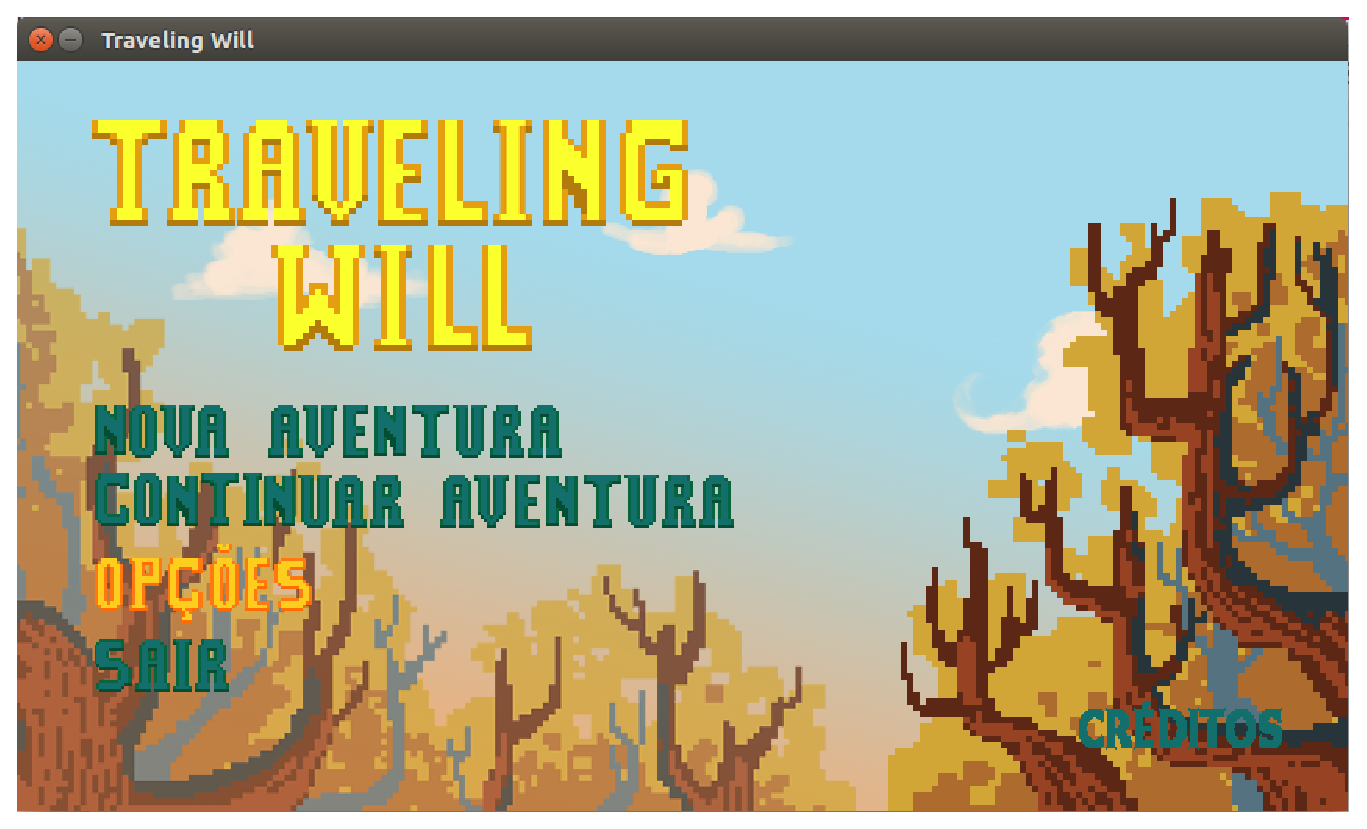
\includegraphics[width=16cm]{figuras/tw-original-1.eps} }}%
    \qquad
    \subfloat[Protótipo sendo executado no emulador de GBA. Fonte: \textit{Autores}.]{{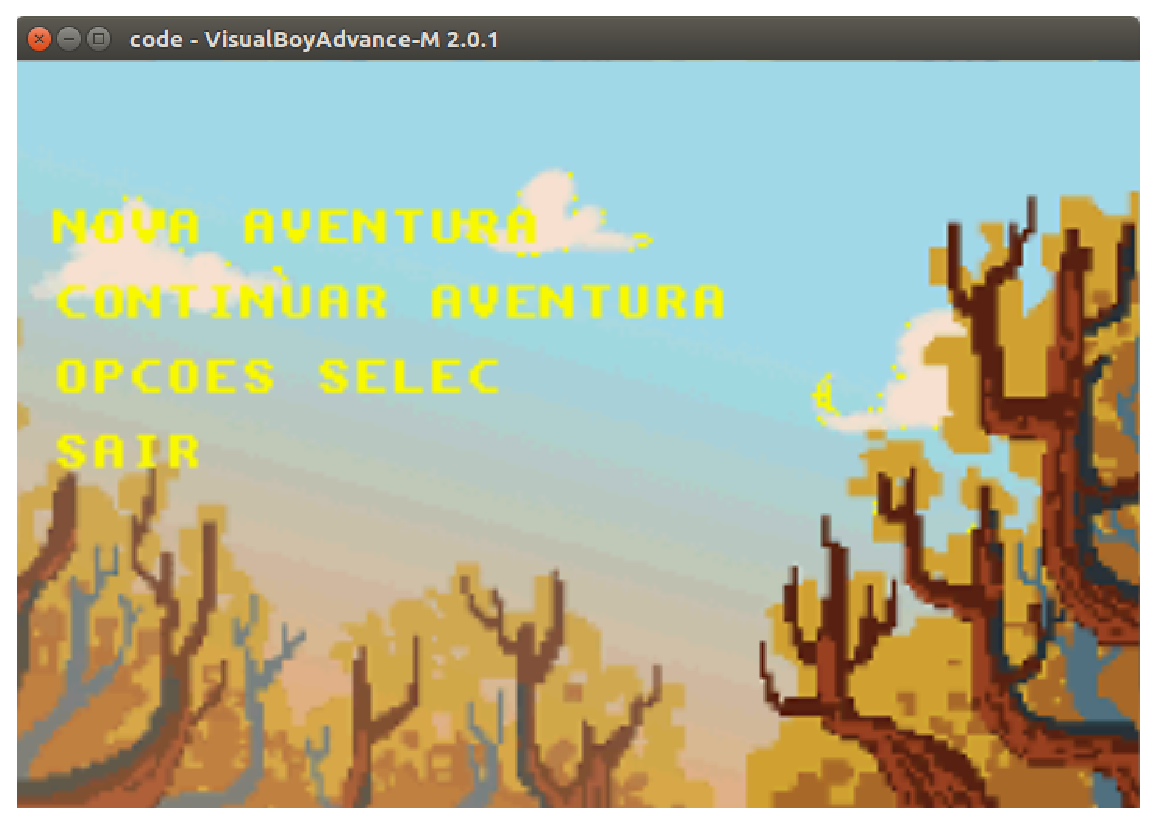
\includegraphics[width=16cm]{figuras/tw-gba-1.eps} }}%
    \caption{Comparação entre o jogo original e o protótipo no emulador.}%
    \label{fig:example}%
\end{figure}

Este protótipo inicial contém apenas a tela vista acima, com um \textit{background} desenhado ao fundo e quatro botões clicáveis, porém sem nenhuma ação após o clique. Para alterar o botão selecionado, basta

O protótipo desenvolvido está disponível no seguinte repositório: \url{https://github.com/traveling-will-gba/traveling-will-prototype}

\section{Desenvolvimento da \textit{engine}}

  Logo após a finalização do protótipo, foi iniciado o desenvolvimento da \textit{engine} responsável por substituir a \textit{libtonc} e gerenciar os recursos do jogo. Esta \textit{engine} contém os seguintes módulos: \textit{input}, vídeo, gerenciador de memória, áudio e física. Além disso, a \textit{engine} contém abstrações para os níveis (\textit{levels}) e objetos do jogo (\textit{game objects}) e um módulo utilitário para funções genéricas relacionadas ao \textit{hardware} do GBA.

  Os módulos de vídeo, \textit{input}, física e as abstrações para níveis e objetos do jogo foram desenvolvidos tendo como base a \textit{ijengine}\footnote{\textit{ijengine}, disponível em \url{https://github.com/fgagamedev/ijengine}}, \textit{engine} desenvolvida para a disciplina de Introdução aos Jogos Eletrônicos, que tem como foco a criação de jogos para PC utilizando \textit{C++}. Ela contém módulos de vídeo, áudio, manipulação de eventos, física, \textit{input}, dentre outros, e contém uma interface para a utilização de diferentes bibliotecas gráficas, como SDL\footnote{\textit{Simple DirectMedia Layer}, disponível em \url{https://www.libsdl.org}} e OpenGL\footnote{OpenGL, disponível em \url{https://www.opengl.org}}.

  \subsection{Módulo de \textit{input}}

Os estados dos botões do GBA ficam salvos em um registrador. Cada um desses estados é representado por um \textit{bit} do valor guardado por esse registrador. Sempre que um botão é pressionado, o GBA automaticamente troca o valor guardado nesse registrador de tal forma que o \textit{bit} que representa o botão em questão passe a possuir valor 0. De forma similar, quando o botão é solto, o valor contido no \textit{bit} em questão é modificado para 1, seu valor padrão. Sendo assim, a checagem dos estados pode ser realizada facilmente utilizando \textit{bitmasks}.

Por exemplo, caso se deseje checar um botão representado pelo \textit{bit} 2 (com a contagem começando em 0), basta pegar o resultado do \textit{AND} binário entre o valor guardado no registrador e a potência de 2 que possui como expoente o \textit{bit} em questão (4, nesse exemplo). No Código \ref{lst:input1} é possível visualizar a definição das constantes que representam os botões. A função utilizada para checar o estado de cada um deles pode ser vista no código \ref{lst:lalala}.

\begin{lstlisting}[caption={Cabeçalho do módulo de \textit{input}.},label={lst:input1}]
#ifndef INPUT_H
#define INPUT_H

#include <stdbool.h>
#include "base_types.h"

#define BUTTON_A 1
#define BUTTON_B 2
#define BUTTON_SELECT 4
#define BUTTON_START 8
#define BUTTON_RIGHT 16
#define BUTTON_LEFT 32
#define BUTTON_UP 64
#define BUTTON_DOWN 128
#define BUTTON_R 256
#define BUTTON_L 512
#define N_BUTTON 10

int pressed_state[N_BUTTON];

void check_buttons_states();
bool pressed(int button);

#endif
\end{lstlisting}

\begin{lstlisting}[caption={Código-fonte do módulo de \textit{input}.},label={lst:lalala}]
#include "input.h"

volatile unsigned int *buttons_mem = (volatile unsigned int *) 0x04000130;

void check_buttons_states() {
    for(int i = 0; i < N_BUTTON; i++) {
        pressed_state[i] = !((*buttons_mem) & (1 << i));
    }
}

bool pressed(int button) {
    return pressed_state[button];
}
\end{lstlisting}

A Figura \ref{demo-input} apresenta o teste implementado para checar o pressionamento dos botões do GBA. Para cada botão pressionado um \textit{pixel} vermelho aparece na tela. Nesta figura, os botões B, R, \textit{LEFT}, \textit{DOWN} e \textit{START} estão sendo pressionados simultaneamente. O código \ref{lst:inputtest} apresenta este teste.

\begin{figure}[H]
 \centering 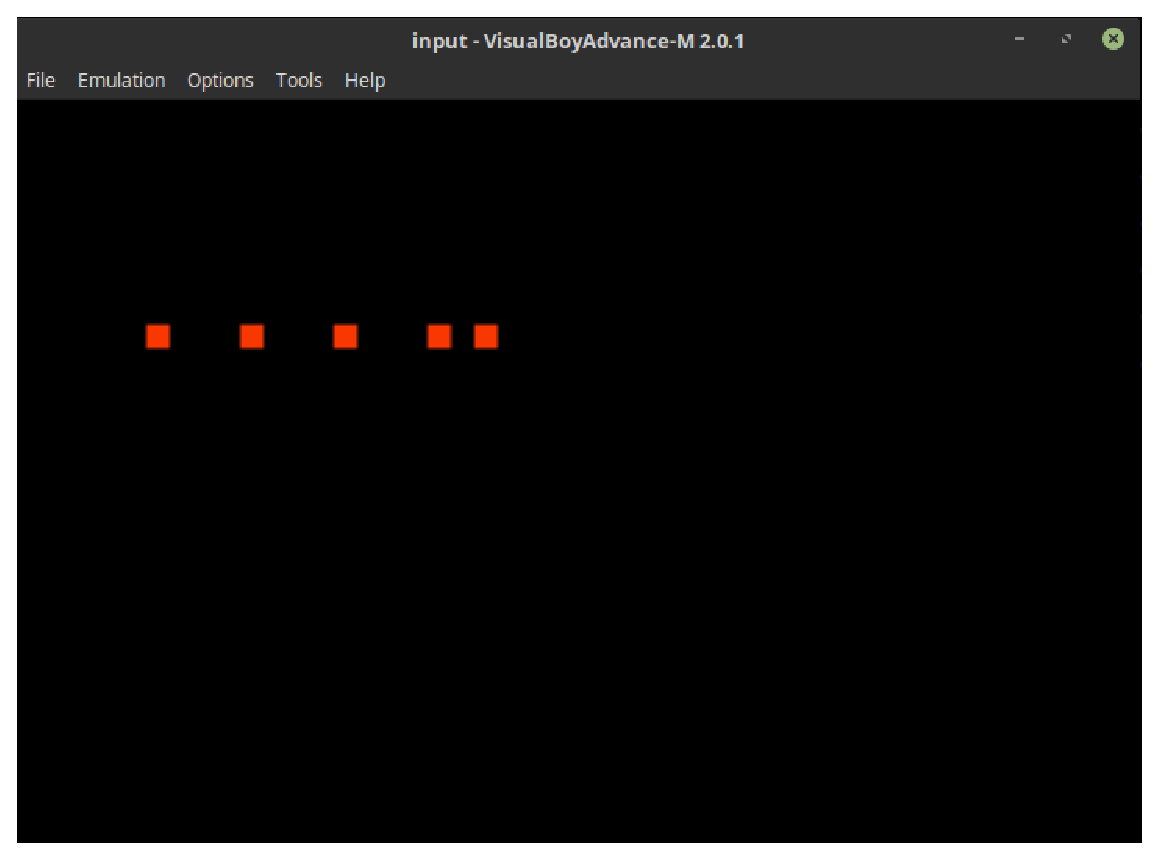
\includegraphics[keepaspectratio=true,scale=0.6]{figuras/demo-input.eps}
   \caption[Demonstração do pressionamento de botões no emulador]
    {Teste de pressionamento de botões no emulador.}
   \label{demo-input}
\end{figure}

\begin{lstlisting}[float,caption={Código de teste de \textit{input}.},label={lst:inputtest}]
#include "video.h"
#include "input.h"

#define RED 0x0000FF

unsigned short *vid_mem = (unsigned short *)0x6000000;

int main() {
    reset_dispcnt();
    set_video_mode(3);
    set_background_number(2);

    while(1) {
        check_buttons_states();

        for(int i=0;i<=9;i++){
            if (pressed(i)) {
                vid_mem[50 * 240 + i * 10] = RED;
            } else {
                vid_mem[50 * 240 + i * 10] = 0;
            }
        }
    }

    return 0;
}
\end{lstlisting}

O código deste projeto se encontra no seguinte endereço: \url{https://bit.ly/2BQV6jf}.

  \subsection{Módulo de vídeo}

O módulo de vídeo é responsável pelo controle do modo de vídeo, dos \textit{backgrounds} e da renderização das \textit{sprites}.

Para gerenciar a renderização das \textit{sprites} foi desenvolvida uma classe chamada \textit{Texture}. Ela foi planejada de forma a não apenas copiar os dados da imagem para a região de memória apropriada, mas também permitir a animação das \textit{sprites} de uma textura e controlar os metadados das imagens renderizadas no jogo.

A seguir, será explicado, com o auxílo de trechos do código, o funcionamento dos principais elementos dessa classe. No código \ref{lst:textureconstructor} é possível visualizar o primeiro construtor. Ele recebe os ponteiros para a paleta de cores e para o vetor de \textit{tiles} utilizados pela imagem, os tamanhos das regiões de memória alocadas pra cada um desses ponteiros e a quantidade de \textit{bits} por \textit{pixel} que a imagem utiliza. Cada um desses atributos é guardado na própria classe, e, já nesse construtor, são chamados os métodos \texttt{set\_sprite\_pal} e \texttt{set\_sprite}, responsáveis por copiá-los para as regiões apropriadas. Por fim, ainda nesse construtor, são atribuídos os índices do \textit{tile base} e da paleta de cores utilizada pela imagem. O cálculo desses índices será explicado logo adiante, nos tópicos dedicados aos métodos \texttt{set\_sprite\_pal} e \texttt{set\_sprite}.

\begin{lstlisting}[float,caption={Construtor da classe \textit{Texture}.},label={lst:textureconstructor}]
Texture::Texture(uint32_t num_sprites, const uint16_t *pallete, uint32_t pallete_len,
    const unsigned int *tiles, uint32_t tiles_len, enum bits_per_pixel bpp = _8BPP)
{
    this->pallete = pallete;
    this->pallete_len = pallete_len;
    this->pallete_id = 0;
    this->bpp = bpp;
    this->num_sprites = num_sprites;
    this->num_tiles = tiles_len / ((bpp == _4BPP) ? 32 : 64);
    this->tiles_per_sprite = num_tiles / num_sprites;
    this->tiles = tiles;
    this->tiles_len = tiles_len;

    memory_manager = MemoryManager::get_memory_manager();

    set_sprite_pal();
    set_sprite();
    oam_entry = memory_manager->alloc_oam_entry();

    metadata.tid = tile_base * ((bpp == _4BPP) ? 1 : 2);
    metadata.pb = pallete_id;
}
\end{lstlisting}

O segundo construtor funciona de forma similar ao anterior, com a diferença de que em vez de receber todos os atributos da imagem, ele recebe apenas um ponteiro para outra textura. Esse construtor serve para quando se deseja renderizar réplicas de uma mesma textura. Utilizar ele permite que tais texturas compartilhem a paleta de cores e o vetor de \textit{tiles}, fazendo-se necessário alocar espaço apenas para os metadados, que são diferentes pra cada textura. Veja o código \ref{lst:copyconstructor}

\begin{lstlisting}[float,caption={Construtor por cópia da classe \textit{Texture}.},label={lst:copyconstructor}]
Texture::Texture(const Texture *texture)
{
    this->num_sprites = texture->num_sprites;
    this->pallete = texture->pallete;
    this->pallete_len = texture->pallete_len;
    this->tiles = texture->tiles;
    this->tiles_len = texture->tiles_len;
    this->bpp = texture->bpp;
    this->pallete_id = texture->pallete_id;
    this->num_tiles = texture->num_tiles;
    this->tiles_per_sprite = texture->tiles_per_sprite;
    this->tile_base = texture->tile_base;

    memory_manager = MemoryManager::get_memory_manager();

    oam_entry = memory_manager->alloc_oam_entry();

    metadata.tid = tile_base * ((bpp == _4BPP) ? 1 : 2);
    metadata.pb = pallete_id;
}
\end{lstlisting}

O método \texttt{set\_sprite\_pal} é responsável por chamar o método \texttt{alloc\_texture\_pal} da classe \texttt{MemoryManager} passando como parâmetro o tamanho da paleta de cores a ser alocada. Como resultado, ele irá receber o endereço de memória aonde a paleta deverá ser guardada. Após fazer a cópia da paleta, é preciso calcular o índice da paleta escolhida na memória, já que esse é um dos metadados necessários para renderização da imagem a 4 \textit{bits} por \textit{pixel}. Como a região reservada para as paletas de cores no \textit{GBA} é dividida em regiões de 32 \textit{bytes}, para realizar tal cálculo basta pegar a diferença entre o início da região escolhida para a cópia e o início da região reservada para as paletas e dividir por 32.
Como uma imagem renderizada a 8 \textit{bits} por \textit{pixel} ocupa toda a região reservada para as paletas, o cálculo do índice não é necessário para uma imagem que utilize 256 cores.

\begin{lstlisting}[float,caption={Função de alocação da paleta de cores de uma textura.}]
bool Texture::set_sprite_pal() {
    volatile uint8_t *teste = memory_manager->alloc_texture_palette(32);
    mem16cpy(teste, pallete, 32);

    this->pallete_id = (teste - (volatile uint8_t *)0x05000200) / 32;

    return true;
}
\end{lstlisting}

O método \texttt{set\_sprite} funciona de forma similar ao \texttt{set\_sprite\_pal}, tendo como diferença relevante apenas o cálculo do índice do \textit{tile\_base} da imagem, que é feito subtraindo o início da região escolhida para a cópia e o início da região reservada para os \textit{tiles}. Essa diferença ocorre porque diferentemente da paleta de cores, cada unidade do vetor que representa a \texttt{tile\_mem} no nosso código é, de fato, um \textit{tile}.

\begin{lstlisting}[float,caption={Função de alocação das \textit{sprites} de uma textura.}]
bool Texture::set_sprite() {
    volatile struct tile *teste = memory_manager->alloc_texture(tiles_len);

    mem16cpy((volatile struct tile *)teste, tiles, tiles_len);
    tile_base = teste - memory_manager->base_texture_mem();

    return true;
}
\end{lstlisting}

O método \texttt{update\_metadata} apenas copia os metadados para a \textit{OAM} (\textit{Object Attributes Memory}).

\begin{lstlisting}[float,caption={Função de cópia dos metadados das texturas.}]
void Texture::update_metadata() {
    mem16cpy(oam_entry, &metadata, sizeof(struct attr));
}
\end{lstlisting}

Por fim, o método \texttt{update} calcula qual a próxima sprite a ser renderizada e atribui o primeiro \textit{tile} dela como \texttt{tile\_id}. Esse processo é o que permite a animação das \textit{sprites} do jogo. O cálculo é feito somando o \texttt{tile\_id} atual com a quantidade de \textit{tiles} por \textit{sprite} da textura que está sendo renderizada. Vale ressaltar que os índices dos \textit{tiles} são contabilizados sempre de 32 em 32 \textit{bytes}, mesmo que a imagem utilize 8 \textit{bits} por \textit{pixel} e por isso o número de \textit{tiles} por \textit{sprite} é multiplicado por 2 quando o número de \textit{bits} por \textit{pixel} da textura é 8.

Para a renderização dos \textit{backgrounds}, foi desenvolvida uma classe que recebe ponteiros para a paleta de cores, para o vetor de \textit{tiles} e para o mapa de \textit{tiles} utilizados pelo \textit{background}, assim como os tamanhos das regiões alocadas pra cada um desses ponteiros. Assim que é instanciada, essa classe calcula qual o melhor \textit{charblock} e o melhor \textit{screenblock} para guardar os \textit{tiles} e o mapa de \textit{tiles}, respectivamente. Vale ressaltar que os \textit{charblocks} e \textit{screenblocks} compartilham a mesma região de memória e precisam de um espaço contíguo na memória do \textit{GBA} para que o \textit{background} seja renderizado corretamente. Por esse motivo não é recomendado apenas copiá-los para a memória do \textit{GBA} de forma sequencial, já que isso poderia causar um \textit{overlap} entre um \textit{charblock} e um \textit{screenblock}, e também poderia preencher a memória do \textit{GBA} de forma não-ótima, o que pode fazer com que não caibam todos os \textit{backgrounds} necessários para uma ou mais fases do jogo.

  \subsection{Módulo gerenciador de memória}

Para melhor utilização dos recursos providos pelo GBA foi desenvolvido um módulo que trata do gerenciamento de memória dos objetos do jogo. A principal responsabilidade deste módulo é garantir que a alocação e desalocação de recursos seja feita de forma eficiente e segura.

    \subsubsection{Funcionamento do gerenciador de memória}

    O modelo de gerenciamento escolhido para ser utilizado neste projeto foi o modelo de gerenciamento com partições variáveis \cite{tanenbaum}. Esse modelo se faz necessário pois os recursos a serem alocados durante a execução do jogo contém tamanhos distintos (uma sprite ocupa menos espaço que um \textit{background} que, por sua vez, ocupa menos espaço do que uma música). Além disso, é importante citar que este gerenciador aloca os recursos contiguamente na memória, isto é, ele sempre irá optar pelo primeiro espaço disponível a partir do começo da memória.

    Utilizando esse modelo como base, o gerenciador funciona da seguinte maneira:

    \begin{itemize}
        \item o construtor do gerenciador de memória é responsável por inicializar todos os ponteiros correspondentes aos endereços dos registradores de \textit{backgrounds}, texturas e atributos das texturas;
        \item quando ocorre uma chamada de alocação, o gerenciador procura pelo primeiro espaço disponível na memória correspondente para alocar tal recurso. Caso não ache nenhum espaço disponível, retorna um endereço nulo;
        \item após achar um endereço disponível, é verificado se há espaço suficiente para alocar o recurso. Caso não haja espaço suficiente, um endereço nulo é retornado;
        \item após garantir que há um espaço disponível e com espaço suficiente para alocação, a posição deste endereço no vetor auxiliar (responsável por indicar se determinado endereço está disponível ou não) é ligada (indicando que o espaço foi ocupado) e é retornado o endereço desta posição para o cliente realizar a cópia do recurso.
    \end{itemize}

    Abaixo segue a função responsável por realizar a alocação de paletas (tanto para \textit{backgrounds} quanto para texturas). Segundo \citeonline{gbatek}, as paletas possuem 256 entradas de 2 \textit{bytes}, totalizando 512 \textit{bytes}.

    \begin{minted}[frame=lines, linenos]
    {c++}
    volatile uint8_t *MemoryManager::alloc_palette(bitset<512>& used,
        volatile uint8_t *palette, size_t size)
    {
        int used_size = used.size();

        for (size_t i = 0; i < used_size; i++) {
            // if this position is taken, skip it
            if (used[i] == true) {
                continue;
            }

            uint32_t available_pal_len = used_size - i;

            // if there is no space to allocate this pallete, skip it
            if (size > available_pal_len) {
                continue;
            }

            // mark positions from i to size as used
            for (size_t j = 0; j < size; j++) {
                used[i + j] = true;
            }

            memory_map[palette + i] = size;

            return palette + i;
        }

        return NULL;
    }
    \end{minted}

    \makebox[\linewidth]{Código de alocação de paletas para \textit{backgrounds} e texturas. Fonte: \textit{Autores}.}
    \vspace{\onelineskip}


    \subsubsection{Gerenciamento seguro de memória}

    Para garantir que novos recursos sejam alocados e que nenhum objeto já carregado na memória seja sobrescrito ou corrompido, qualquer chamada que envolva a alocação de novos recursos passa por um processo onde é verificado se a memória que será populada contém espaço suficiente realizar tal alocação. Para realizar esta verificação, o gerenciador possui um mapa que associa um endereço na memória com o tamanho que o objeto alocado neste endereço ocupa. Deste modo, quando há uma chamada de alocação com tamanho \textit{size} e uma posição \textit{i} está disponível, as posições de \textit{i} até \textit{i + size / (tamanho de cada partição da memória correspondente em bytes) - 1} são marcadas como utilizadas.

    \subsubsection{Gerenciamento eficiente de memória}

    As estratégias utilizadas para garantir um gerenciamento eficiente de memória envolvem a utilização de \textit{singleton} para a criação do objeto gerenciador de memória e  utilização de estruturas de dados que permitam configurar o tamanho a ser utilizado.

    \begin{itemize}
        \item \textbf{Utilização de \textit{singleton} para o gerenciador de memória}: Para que haja um único objeto encarregado de gerenciar a alocação de recursos no jogo, a classe \textit{MemoryManager} foi modelada utilizado o padrão de projeto \textit{Singleton}. Com este padrão de projeto, cada chamada de criação de uma nova instância do gerenciador de memória passa por uma verificação, que checa se já existe uma instância desta classe (por meio de uma variável dentro da própria classe que armazena uma instância de \textit{MemoryManager} ou nulo). Caso haja, esta instância é retornada. Caso contrário, é criada uma nova instância. Segue o código exemplificando o \textit{singleton} (trechos de código desta classe foram omitidos para melhor foco no padrão de projeto):

        \begin{minted}[frame=lines, linenos]
        {c++}
        class MemoryManager {
            private:
                MemoryManager *instance;

            public:
                MemoryManager *get_memory_manager() {
                    if (!instance) {
                        instance = new MemoryManager();
                    }

                    return instance;
                }
        };
        \end{minted}
        \makebox[\linewidth]{\textit{Singleton} do gerenciador de memória. Fonte: \textit{Autores}.}
        \vspace{\onelineskip}


        \item \textbf{Estruturas de dados apropriadas para configuração de tamanho utilizado}: A fim de não utilizar memória desnecessariamente, em alguns pontos do jogo foram utilizadas estruturas que permitem configurar a quantidade de \textit{bits} que podem ser utilizados por cada variável. O primeiro exemplo mostra uma \textit{struct} que armazena os atributos das texturas, onde cada atributo só precisa de um pequeno número de bytes. Já o segundo exemplo demonstra a utilização de \textit{bitsets} (que mantém a disponibilidade de cada posição do endereço de memória) com tamanho fixo correspondente ao tamanho total da respectiva região de memória (neste exemplo, \textit{Object Attribute Memory}).

        \begin{minted}[frame=lines, linenos]
        {c++}
        struct attr {
            uint8_t y;
            uint8_t om : 2;
            uint8_t gm : 2;
            uint8_t mos : 1;
            uint8_t cm : 1;
            uint8_t sh : 2;

            uint16_t x : 9;
            uint8_t aid : 5;
            uint8_t sz : 2;

            uint16_t tid : 10;
            uint8_t pr : 2;
            uint8_t pb : 4;

            uint16_t filler;
        };
        \end{minted}
        \makebox[\linewidth]{\textit{Struct} com \textit{bitfields} para atributos das texturas. Fonte: \textit{Autores}.}
        \vspace{\onelineskip}

        \begin{minted}[frame=lines, linenos]
        {c++}
        // backgrounds and textures have 512 bytes each for palette memory
        bitset<512> background_palette_used;
        bitset<512> texture_palette_used;

        // max number of charblocks that can be stored in VRAM
        bitset<4> charblock_used;
        // max number of screenblocks that can be stored in VRAM
        bitset<32> screenblock_used;
        \end{minted}
        \makebox[\linewidth]{\textit{Bitsets} para checagem de disponibilidade na memória. Fonte: \textit{Autores}.}
        \vspace{\onelineskip}

    \end{itemize}

  \subsection{Módulo de Física}

O módulo de física é responsável por checar continuamente se os objetos estão colidindo e caso estejam chamar as funções responsáveis por lidar com a colisão para cada objeto. Para realizar tal procedimento esse módulo guarda uma lista de objetos que devem ser considerados na checagem e um ponteiro para o objeto alvo. Dessa forma, sempre que algum objeto colide com o objeto alvo, o método \texttt{on\_collision()} do alvo e do objeto com o qual ele colidiu é chamado.


A \textit{engine} desenvolvida está disponível no seguinte repositório: \url{https://bit.ly/2GaTaX1}

  \subsection{Módulo Utilitário}

Este módulo contém funções utilitárias que estão relacionadas diretamente com \textit{hardware} do GBA.

A primeira delas é a função \texttt{print}. Esta função é necessária pois, diferentemente de um programa executado em um PC, a ROM não possui redirecionamento de \textit{output} para uma saída padrão. Após diversas buscas em fóruns de desenvolvimento para GBA, foi encontrada uma solução que permite realizar o redirecionamento do \textit{output buffer} para a saída padrão (\textit{stdin}). A solução consiste em um código \textit{Assembly} que contém uma chamada de sistema \texttt{vbaprint}. O código \ref{lst:vbaprint} apresenta a implementação \textit{Assembly} mencionada.

\begin{lstlisting}[label={lst:vbaprint}, caption={Código \textit{Assembly} para a função \texttt{vbaprint}}]
.arm
.global vbaprint
.type   vbaprint STT_FUNC
.text
vbaprint:
    swi 0xFF0000
        bx lr
\end{lstlisting}

Após isso é necessário declarar a função \texttt{vbaprint} em um cabeçalho em C. O código \ref{lst:vbaprintheader} apresenta este cabeçalho.

\begin{lstlisting}[label={lst:vbaprintheader}, caption={Cabeçalho da função \texttt{vbaprint}}]
#ifndef VBAPRINT_H
#define VBAPRINT_H

extern "C" void vbaprint(const char *message);

#endif
\end{lstlisting}

A implementação da função \texttt{print} utiliza o mesmo modelo de implementação da função \texttt{printf} da linguagem C. Ela recebe como parâmetros uma string e um \textit{wildcard} que indica que esta função recebe um número variável de parâmetros. Esse parâmetros variáveis são guardados em uma variável do tipo \texttt{va\_list}. Para realizar o \textit{parse} da \textit{string} recebida é utilizada a função \texttt{vsnprintf}, que recebe a lista de parâmetros e faz a resolução das variáveis na \textit{string} e retorna a string com as substituições feitas. Após isso, é chamada a função \texttt{vbaprint} que se encarrega de escrever o buffer recebido na saída padrão. O código \ref{lst:utilsprint} apresenta a implementação da função \texttt{print}.

\begin{lstlisting}[float,caption={Implementação da função \texttt{print}},label={lst:utilsprint}]
int print(const char *fmt, ...) {
    va_list args;
    va_start(args, fmt);

    char buffer[4096];

    int rc = vsnprintf(buffer, sizeof(buffer), fmt, args);

    vbaprint(buffer);
    va_end(args);

    return rc;
}
\end{lstlisting}

A próxima função utilitária é a \texttt{mem16cpy}. Esta função funciona de forma similar à função \texttt{memcpy} da linguagem C, porém, copia os dados de uma área de memória para outra 2 \textit{bytes} por vez. Isso se faz necessário pois

TODO

O código \ref{lst:mem16cpy} apresenta a implementação da função \texttt{mem16cpy}.

\begin{lstlisting}[caption={Implementação da função \texttt{mem16cpy}},label={lst:mem16cpy}]
void mem16cpy(volatile void *dest, const void *src, size_t n)
{
    if (n & 1) {
        print("Size must be even");
    }

    for (int i = 0; i < n / 2; i++) {
        *(((volatile uint16_t *)dest) + i) = *(((uint16_t *)src) + i);
    }
}
\end{lstlisting}

A última função deste módulo utilitário é a \texttt{vsync} (\textit{vertical synchronization}). Ela tem como responsabilidade servir como um mecanismo para garantir a atualização do jogo durante o período de VBlank (período onde há uma pausa na atualização vertical da tela do jogo). O código \ref{lst:vsync} apresenta a implementação do \texttt{vsync}.

\begin{lstlisting}[caption={Implementação da função \texttt{vsync}},label={lst:vsync}]
void vsync() {
    while(REG_VCOUNT >= 160);
    while(REG_VCOUNT < 160);
}
\end{lstlisting}

  \subsection{Abstrações de níveis e objetos do jogo}

Além de implementar módulos relacionados a entrada (\textit{input}) e saída (vídeo, áudio, entre outros), a \textit{engine} também implementa abstrações para os níveis e para os objetos do jogo.

Os \textit{game objects} são a base para qualquer elemento utilizado no jogo. Um \textit{game object} possui uma posição \texttt{(x, y)} no espaço do jogo, possui velocidade horizontal e vertical, possui \textit{game objects} filhos (que formam uma hierarquia de \textit{game objects}) e tem como responsabilidades atualizar seu próprio estado, se desenhar na tela e atualizar os seus filhos.

Pelo fato de o mecanismo de renderização ser, de certa forma, automático (basta carregar as imagens na memória e especificar os metadados que elas já são renderizadas na tela), a função de se desenhar na tela não é utilizada. Porém, a atualização e controle dos filhos é importante para o comportamento correto desses objetos. O código \ref{lst:gameobj} apresenta a classe \texttt{GameObject}.

\begin{lstlisting}[label={lst:gameobj},caption={Classe \texttt{GameObject}}]
#ifndef GAME_OBJECT_H
#define GAME_OBJECT_H

#include <vector>
#include <stdint.h>

using std::vector;

class GameObject {
    protected:
        GameObject *m_parent;
        int m_x, m_y;
        int m_speed_x, m_speed_y;
        vector <GameObject *> m_children;

        GameObject *parent() const { return m_parent; }

        virtual void update_self(uint64_t dt) = 0;
        virtual void draw_self() = 0;

    public:
        void update(uint64_t dt);
        void draw();

        void set_parent(GameObject *obj) { m_parent = obj; }
        void add_child(GameObject *);
        void remove_child(GameObject *);
};

#endif
\end{lstlisting}

Com a definição e implementação dos \textit{game objects}, a caracterização da abstração dos níveis do jogo se torna bem simples. De forma geral, um nível é um \textit{game object} que, além de possuir todas as propriedades já explicitadas acima, possui uma variável que indica se o nível foi finalizado e outra que guarda o próximo nível a ser renderizado. O código \ref{lst:level} apresenta a implementação da classe \texttt{Level}.

\begin{lstlisting}[label={lst:level},caption={Classe \texttt{Level}}]
#ifndef LEVEL_H
#define LEVEL_H

#include "game_object.h"

#include <stdio.h>

class Level : public GameObject {
    protected:
        int m_x, m_y;
        bool m_done;
        int m_next;
};

#endif
\end{lstlisting}

\section{Desenvolvimento do jogo}

  De acordo com o cronograma apresentado na versão anterior, as funcionalidades do jogo original que foram planejadas para a realização deste trabalho são:

  \begin{itemize}
    \item F1: implementação do menu principal do jogo
    \item F2: implementação da rolagem infinita dos \textit{backgrounds}
    \item F3: implementação do mecanismo de renderização das plataformas
    \item F4: implementação da movimentação do personagem principal
    \item F5: implementação do mecanismo de renderização dos itens coletáveis
    \item F6: implementação das telas de finalização dos níveis
    \item F7: carregamento dos níveis a partir do \textit{level design}
    \item F8: implementação do seletor de fases
    \item F9: implementação das opções do menu
    \item F10: implementação do tutorial
  \end{itemize}

  Da lista acima, as funcionalidades \texttt{F8}, \texttt{F9} e \texttt{F10} foram removidas da realização do projeto.

  O desenvolvimento do jogo foi marcado por quatro fases principais (que ocorreram simultaneamente): adaptação das imagens do jogo, construção dos níveis do jogo, transição entre os níveis do jogo e adaptação das músicas do jogo.

  \subsection{Adaptação das imagens do jogo} \label{adapak}

Esta fase foi marcada principalmente pelo entendimento de como imagens são carregadas e interpretadas pelo GBA.

Primeiramente, era necessário conhecer a resolução das imagens no jogo original e no jogo a ser portado para que pudesse ser estabelecida uma proporção a ser utilizada na adaptação das imagens. Para isso, foram utilizadas as imagens de \textit{background}, pois elas ocupam todo o espaço da janela do jogo original. A altura dos \textit{backgrounds} no jogo original é \textit{480px} e, sabendo que a tela do GBA possui \textit{160px}, é possível estabelecer um fator de conversão bastante preciso, seguindo a fórmula

\begin{equation}
\label{Cálculo da proporção das imagens do jogo}
\frac{480_{px}}{160_{px}} = \frac{3}{1}
\end{equation}

Portanto, a proporção das imagens do jogo original para o jogo a ser portado é de \texttt{3:1}.

Após realizar o redimensionamento das imagens para o tamanho correto, foi necessário descobrir como utilizar essas imagens no GBA. Diferentemente de sistemas mais modernos, o GBA não carrega imagens de fato, e sim um código C que contém as informações da imagem, como paleta de cores, \textit{tiles} e o mapeamento desses \textit{tiles} na imagem. Para realizar a conversão da imagem para este código, foi utilizada a ferramenta GRIT (\textit{GBA Raster Image Transmogrifier}). Com essa ferramenta é possível converter a imagem utilizando uma série de parâmetros, como quantidade de bits por pixel da imagem, formato de redução de \textit{tiles}, formato de saída do arquivo gerado (C, \textit{Assembly}, entre outros), altura e largura, em \textit{tiles} (conjuntos de \textit{8px} x \textit{8px}), da imagem , dentre outras opções. Para a conversão das \textit{sprites} do jogo, o seguinte comando foi utilizado:

\begin{lstlisting}[language=bash,caption={Comando para conversão das imagens em código}]
$ grit nome-da-imagem.png -gB4 -ftc -Mw2 -Mh4
\end{lstlisting}

Nesse comando, o código relativo à imagem é gerado considerando que cada \textit{pixel} da imagem utiliza 4 \textit{bits} (\texttt{-gb4}), exportando a imagem como código C (\texttt{-ftc}) e definindo a largura e a altura da imagem como sendo, respectivamente, \textit{16px} (\texttt{-Mw2}) e \textit{32px} (\texttt{-Mh4}). O resultado da execução dessa instrução é um \textit{header} e um código-fonte correspondentes à imagem, contendo uma paleta com as cores utilizadas e um vetor de \textit{tiles}, assim como mostrado nos códigos \ref{lst:imageheader} e \ref{lst:imagecpp}.


\begin{lstlisting}[caption={Cabeçalho da parte superior da imagem da plataforma da primeira fase.},label={lst:imageheader}]
//{{BLOCK(level1_plat0)

//======================================================================
//
//  level1_plat0, 16x32@4,
//  Transparent palette entry: 17.
//  + palette 16 entries, not compressed
//  + 8 tiles Metatiled by 2x4 not compressed
//  Total size: 32 + 256 = 288
//
//  Time-stamp: 2018-11-28, 22:18:37
//  Exported by Cearn's GBA Image Transmogrifier, v0.8.15
//  ( http://www.coranac.com/projects/#grit )
//
//======================================================================

#ifndef GRIT_LEVEL1_PLAT0_H
#define GRIT_LEVEL1_PLAT0_H

#define level1_plat0TilesLen 256
extern const unsigned int level1_plat0Tiles[64];

#define level1_plat0PalLen 32
extern const unsigned short level1_plat0Pal[16];

#endif // GRIT_LEVEL1_PLAT0_H

//}}BLOCK(level1_plat0)
\end{lstlisting}

\begin{lstlisting}[caption={Código fonte da parte superior da imagem da plataforma da primeira fase.},label={lst:imagecpp}]
//{{BLOCK(level1_plat0)

//======================================================================
//
//  level1_plat0, 16x32@4,
//  Transparent palette entry: 17.
//  + palette 16 entries, not compressed
//  + 8 tiles Metatiled by 2x4 not compressed
//  Total size: 32 + 256 = 288
//
//  Time-stamp: 2018-11-28, 22:18:37
//  Exported by Cearn's GBA Image Transmogrifier, v0.8.15
//  ( http://www.coranac.com/projects/#grit )
//
//======================================================================

const unsigned int level1_plat0Tiles[64] __attribute__((aligned(4))) __attribute__((visibility("hidden")))=
{
    0xCCCCCCCC,0xAAACCCCC,0x888AACCB,0x89988BBA,0x99889888,0x99898221,0x98822222,0x81122444,
    0xCCCCCCCC,0xCCCCCCBA,0xCCCCCA89,0xBB888989,0x78888988,0x25889988,0x44225889,0x22444168,
    0x22244223,0x44444444,0x44444444,0x44444444,0x44444444,0x44444444,0x44444444,0x44444444,
    0x44223432,0x44444244,0x44444444,0x44444444,0x44444444,0x44444444,0x44444444,0x44444444,
    0x44444444,0x44444444,0x44444444,0x43344334,0x24422222,0x42222222,0x22222222,0x22222222,
    0x44444444,0x44444444,0x44444444,0x33444344,0x44223432,0x22444244,0x22222222,0x11222222,
    0x22222222,0x21122222,0x11111111,0x11111111,0x11111111,0x11111111,0x11111111,0x11111111,
    0x11222222,0x11111122,0x11111111,0x11111111,0x11111111,0x11111111,0x11111111,0x11111111,
};

const unsigned short level1_plat0Pal[16] __attribute__((aligned(4))) __attribute__((visibility("hidden")))=
{
    0x0002,0x0889,0x088B,0x088D,0x10D0,0x092D,0x09AD,0x0A50,
    0x0A90,0x1290,0x0AD0,0x1332,0x1B74,0x0000,0x0000,0x0000,
};

//}}BLOCK(level1_plat0)
\end{lstlisting}

Já para a conversão das imagens dos \textit{backgrounds} foi utilizado o seguinte comando:

\begin{lstlisting}[language=bash,caption={Comando para conversão dos \textit{backgrounds} em código}]
$ grit nome-da-imagem.png -gB4 -ftc -mRtf -mp0
\end{lstlisting}

Assim como na imagem anterior, o código é gerado em C considerando que cada \textit{pixel} da imagem utiliza 4 \textit{bits}. Além disso, o código é gerado utilizando redução completa de \textit{tiles} (\texttt{-mRtf}) e, diferentemente das sprites, onde o índice a ser utilizado na paleta de cores é especificado apenas no código, é necessário especificar, já nessa instrução (\texttt{-mp0}), o índice da paleta de cores que será utilizada no código para guardar as cores da imagem. Vale ressaltar que isso é necessário apenas caso a imagem esteja sendo convertida a 4 \textit{bits} por \textit{pixel}, já que a 8 \textit{bits} por \textit{pixel} é possível utilizar apenas uma única paleta de cores, assim como já explicado na seção \ref{gba-memory}.

Nesse ponto da explicação é necessário saber diferenciar 3 coisas: o \textit{background} do GBA, as imagens que irão compor o \textit{background} do jogo e o que de fato vai ser mostrado na tela. O \textit{background} do GBA é todo o espaço disponível para o mapa do jogo, ele determina os limites do jogo. Se ele tiver \textit{512px} de largura, os limites horizontais do mapa irão de 0 a 512. Esse será o espaço disponível para carregamento de todo e qualquer elemento do jogo, seja ele \textit{sprite} ou imagem de fundo. Porém, nem tudo que estiver carregado no \textit{background} do GBA será necessariamente mostrado na tela, afinal a tela do GBA possui apenas \textit{240px} de largura e \textit{160px} de altura. O que será de fato mostrado dependerá do que será explicado à frente.

Nos modos de vídeo baseados em \textit{tiles}, o GBA possui um total de 4 \textit{backgrounds}, sendo que existem restrições explícitas para o tamanho de cada um deles. As dimensões aceitas são as seguintes: 256x256, 512x256, 256x512, 512x512. Cada um desses \textit{backgrounds} possui um registrador por meio do qual é possível escolher suas dimensões. A escolha das dimensões é feita por meio de uma \textit{flag} atribuída diretamente no registrador \texttt{REG\_BGxCNT}. Cada um desses \textit{backgrounds} pode possuir um tamanho diferente, desde que siga as restrições já citadas.

Para passar a ideia de que o personagem está se movimentando durante o jogo, as imagens dos \textit{backgrounds} se movem horizontalmente em velocidades diferentes, técnica chamada \textit{parallax}. Fazer isso convertendo a imagem em uma maior, a replicando em um editor de imagens para posteriormente carregá-la por completo no código provavelmente funcionaria em uma plataforma atual. Porém, no GBA, onde a memória é extremamente limitada, não seria possível nem mesmo carregar tal imagem e mesmo em uma plataforma atual muita memória seria gasta desnecessariamente. Por isso, para realizar essa movimentação, os \textit{backgrounds} do jogo são reproduzidos mudando o ponto onde a renderização começa, sendo que sempre que o \textit{background} chega ao fim, a renderização continua do início. E aqui é importante ressaltar que é o fim do \textit{background} do GBA e não das imagens, por isso é importante que as imagens possuam os mesmos tamanhos dos \textit{backgrounds} em que estão sendo renderizadas nos eixos aonde a movimentação ocorre. Por exemplo, em um \textit{background} de 512x256, em que a imagem de fundo se move somente no sentido horizontal, é necessário que essa imagem de fundo possua \textit{512px} de largura, porém para a altura, basta que a imagem possua a altura da tela, já que ela não será movimentada na vertical e por isso os \textit{pixels} da parte de cima nunca serão vistos.

Na versão original do jogo, o movimento dos \textit{backgrounds} também é realizado dessa forma, porém tendo que manualmente (no código), manipular os índices onde a renderização inicia para passar a ideia de que o \textit{background} é infinito. O GBA facilita esse processo, pois possui registradores que sinalizam o ponto onde acontece o início da renderização da imagem e quando a imagem chega ao fim, ele automaticamente emenda o fim com o início. Dessa forma, se a imagem possuir \textit{256px} de largura, basta que o valor contido no registrador seja continuamente incrementado, sem que seja necessário resetar o valor quando a imagem chegar no seu limite. Outra vantagem que o GBA proporciona ao realizar essa movimentação dos \textit{backgrounds} é o fato de que não há tamanho mínimo para a interseção entre o fim e o início da imagem. Na versão original, por exemplo, em que a resolução era de \textit{852px x 480px}, era necessário que os \textit{852px} finais da imagem fossem iguais aos \textit{852px} iniciais, pois assim, quando o índice do fundo fosse resetado, isso não seria vísivel para quem está jogando, passando a ideia de continuidade. Esse fator facilitou até mesmo a edição das imagens, fazendo com que o \textit{background} pudesse ser mais diverso, sem que fosse necessário gastar grande parte do fim da imagem apenas replicando o início. No código \ref{lst:update_bg}, é possível visualizar uma amostra de como é feita a atualização dos índices. É importante ressaltar que esse efeito da renderização continuar no início acontece para qualquer textura, e não apenas com os mapas. Sendo assim, uma \textit{sprite} cujas extremidades ultrapassem algum dos limites do \textit{background} aonde ela está sendo renderizada (o mais à frente) terá a parte que ultrapassou o \textit{background} renderizada no lado oposto.

\begin{lstlisting}[caption={Método responsável por atualizar os índices de renderização do \textit{background}},label={lst:update_bg}]
void Background::update_self(uint64_t dt) {
    if (dt % frames_to_skip == 0) {
        m_x += m_speed_x;
        m_y += m_speed_y;
    }

    switch(this->background_id) {
        case 0:
            REG_BG0HOFS = m_x;
            REG_BG0VOFS = m_y;
            break;
        case 1:
            REG_BG1HOFS = m_x;
            REG_BG1VOFS = m_y;
            break;
        case 2:
            REG_BG2HOFS = m_x;
            REG_BG2VOFS = m_y;
            break;
        case 3:
            REG_BG3HOFS = m_x;
            REG_BG3VOFS = m_y;
            break;
        default:
            print("Invalid background id\n");
            break;
    }
}
\end{lstlisting}

Dessa forma, sempre que a variável \texttt{m\_x}, que representa o ponto no eixo X onde começa a renderização do \textit{backgrounds} na tela, é atualizado, o registrador correspondente também é atualizado. O mesmo se aplica à variável \texttt{m\_y}, que representa o ponto no eixo Y.

Na versão original do jogo, as imagens das plataformas possuíam \textit{20px} de largura e \textit {400px} de altura. Porém, o GBA possui explícitas limitações em relação às dimensões das imagens a serem renderizadas. Sendo assim, é necessário que as imagens estejam em uma das dimensões mostradas na tabela \ref{table:sprite-sizes}. Tendo em vista que a altura máxima de uma \textit{sprite} no GBA é \textit{64px}, foi necessário dividir a imagem em várias para que fosse possível atingir a altura necessária das plataformas no jogo. As dimensões escolhidas para essas novas imagens foram \textit{16px} de largura por \textit{32px} de altura, pois assim a largura ficava mais próxima da largura original, preservando ao máximo o \textit{level design} original. Já a altura de \textit{32px} foi escolhida tendo em vista que é a altura máxima que pode ser utilizada com largura \textit{16px}, como mostrado na tabela \ref{table:sprite-sizes}.

\begin{table}[htb]
\center
\begin{tabular}{|l|l|l|l|}
\hline
8x8  & 16x16 & 32x32 & 64x64 \\ \hline
16x8 & 32x8  & 32x16 & 64x32 \\ \hline
8x16 & 8x32  & 16x32 & 32x64 \\ \hline
\end{tabular}
\caption{Dimensões válidas para renderização de \textit{sprites} no GBA}
\label{table:sprite-sizes}
\end{table}

Devido a essa adaptação das plataformas, a classe \texttt{TWPlatform} possui um número variável de texturas diferentemente das classes que representam os demais objetos do jogo, que possuem uma única textura. As plataformas podem utilizar uma textura (caso das plataformas que representam o chão, pois apenas a parte mais superior das plataformas é mostrada) ou por 4 texturas, podendo atingir uma altura máxima de \textit{128px}, correspondendo a 80\% da altura da tela do GBA. O código \ref{lst:platform-textures} apresenta o trecho responsável por carregar as texturas e o código \ref{lst:platform-set-y} o trecho responsável por calcular as alturas de cada uma das texturas.

\begin{lstlisting}[caption={\texttt{std::vector} com as texturas das plataformas sendo preenchido.},label={lst:platform-textures}]
m_textures.push_back(new Texture(1, level1_plat0Pal, level1_plat0PalLen, level1_plat0Tiles, level1_plat0TilesLen, _4BPP));
if (not m_is_floor)
{
    m_textures.push_back(new Texture(1, level1_plat1Pal, level1_plat1PalLen, level1_plat1Tiles, level1_plat1TilesLen, _4BPP));
    m_textures.push_back(new Texture(1, level1_plat2Pal, level1_plat2PalLen, level1_plat2Tiles, level1_plat2TilesLen, _4BPP));
    m_textures.push_back(new Texture(1, level1_plat3Pal, level1_plat3PalLen, level1_plat3Tiles, level1_plat3TilesLen, _4BPP));
}
\end{lstlisting}

\begin{lstlisting}[caption={Cálculo das alturas das texturas utilizadas nas plataformas},label={lst:platform-set-y}]
void TWPlatform::set_y(int y) {
    m_y = y;

    for (size_t i = 0; i < m_textures.size(); i++) {
        m_textures[i]->metadata.y = m_y + platform_height * i;

        if (m_y + platform_height * (i + 1) >= 256) {
            // hide sprite
            m_textures[i]->metadata.om = 2;
        } else {
            m_textures[i]->metadata.om = 0;
        }
    }
}
\end{lstlisting}

No código \ref{lst:platform-textures}, uma única textura é carregada caso a plataforma faça parte do chão do jogo e 4 plataformas são carregadas caso contrário. A variável \texttt{m\_is\_floor} indica se a plataforma faz ou não parte do chão.

No código \ref{lst:platform-set-y}, é possível ver que a variável \texttt{m\_y} representa o ponto \texttt{y} (ponto onde a plataforma começa a ser renderizada na tela) da plataforma em si e por isso é utilizado para calcular o \texttt{y} de cada uma das texturas utilizadas na classe.

Ao falar sobre a adaptação do \textit{background}, foi explicado que o GBA automaticamente emenda o fim e o início da tela de fundo, a medida que o ponto onde a renderização da imagem é avançado. O mesmo funciona com as demais imagens do jogo. Sempre que uma imagem ultrapassa as dimensões do \textit{background}, ela começa a ser renderizada no lado oposto. Por exemplo, levando em consideração uma altura de \textit{256px} para o \textit{background} e lembrando que a altura da tela do GBA é de \textit{160px}, se uma imagem de \textit{32px} for renderizada no ponto \texttt{y = 150} na tela, os \textit{22px} restantes serão renderizados a partir do topo do \textit{background}, o que não necessariamente significa que esses \textit{pixels} remanescentes serão mostrados na tela, isso pelo fato de serem carregados na tela apenas os \textit{160px} finais da imagem do \textit{background}. Isso se torna um problema, porém, quando o número de \textit{pixels} que ultrapassam os limites inferiores da tela do GBA são suficientes para alcançar os \textit{160px} finais do \textit{background} e é para isso que serve o trecho que vai da linha 7 à linha 12 no código \ref{lst:platform-set-y}. Este trecho esconde a textura caso ela ultrapasse o limite inferior do \textit{background} (independente de chegar ou não ao ponto do restante da imagem ser renderizado na parte de cima da tela) e mostra caso contrário.


  \subsection{Construção dos níveis do jogo}

A construção dos níveis do jogo tem como base o \textit{level design} desenvolvido para cada nível do jogo original. Este \textit{level design} possui a seguinte estrutura:

\begin{lstlisting}[caption={Estrutura do \textit{level design} do jogo original}]
level_tempo
num_platforms num_backgrounds
platform_height is_enemy_present [enemy_type enemy_height] is_collectable_present [collectable_height]
\end{lstlisting}

A primeira linha do \textit{level design} contém a velocidade da música que será reproduzida no nível. A linha abaixo contém dois valores: número de plataformas e de \textit{backgrounds} do nível. Após isso, seguem \texttt{num\_platform} linhas caracterizando cada plataforma: sua altura, se possui um inimigo, tipo e altura do inimigo (caso haja um inimigo), se possui coletável, altura do coletável (caso haja um coletável).

O bloco \ref{lst:leveldesignexample} mostra um trecho do level design da primeira fase do jogo original

\begin{lstlisting}[label={lst:leveldesignexample},caption={Exemplo do \textit{level design} da fase 1 do jogo original}]
100
220 3
50 0 0
50 0 0
50 0 0
50 0 0
50 0 0
50 0 0
50 0 0
115 0 1 155
115 0 0
115 0 0
111 0 0
111 0 1 151
111 0 0
111 0 0
111 0 0
111 0 1 155
111 0 0
111 0 0
111 0 0
111 0 1 151
...
\end{lstlisting}

Para que o \textit{level design} consiga ser lido e utilizado no jogo portado, foi necessário criar um \textit{parser} do \textit{level design} original para um formato legível no GBA. O \textit{parser} tem como responsabilidade ler o arquivo de \textit{level design} e criar vetores de inteiros correspondentes a: altura das plataformas, presença de inimigo, tipo do inimigo, altura do inimigo, presença de coletável e altura do coletável. O código \ref{lst:levelparser} apresenta o \textit{script python} criado para realizar o \textit{parser} e os códigos \ref{lst:parsedheader} e \ref{lst:parsedcpp} mostram o resultado do \textit{parse}.

\begin{lstlisting}[language=python,label={lst:levelparser},caption={\textit{script python} para realizar o \textit{parse}}]
import sys

if len(sys.argv) < 3:
    print("File name and level_design path must be passed as arguments")
    sys.exit()

file_name = sys.argv[1]
level_design_path = sys.argv[2]

f = open(level_design_path, "r")

header_file = open("{}.h".format(file_name), "w")

level_tempo = f.readline()
level_len, background_num = f.readline().split()

header_file.write("#ifndef {}_H\n".format(file_name.upper()))
header_file.write("#define {}_H\n\n".format(file_name.upper()))
header_file.write("#define {}_tempo {}\n".format(file_name, level_tempo))
header_file.write("#define {}_len {}\n".format(file_name, level_len))

header_file.write("extern const int {}_platform_heights[{}];\n".format(file_name, str(level_len)))
header_file.write("extern const int {}_enemy_present[{}];\n".format(file_name, str(level_len)))
header_file.write("extern const int {}_enemy_type[{}];\n".format(file_name, str(level_len)))
header_file.write("extern const int {}_enemy_heights[{}];\n".format(file_name, str(level_len)))
header_file.write("extern const int {}_collectable_present[{}];\n".format(file_name, str(level_len)))
header_file.write("extern const int {}_collectable_heights[{}];\n".format(file_name, str(level_len)))

header_file.write("\n#endif")

heights = []
ep = []
et = []
eh = []
cp = []
ch = []

for line in f.readlines():
    args = line.split()

    platform_height = 0
    enemy_present = False
    enemy_type = 0
    enemy_height = 0
    collectable_present = False
    collectable_height = 0

    if len(args) == 0:
        continue

    platform_height = args[0]
    enemy_present = int(args[1])

    if enemy_present:
        enemy_type = args[2]
        enemy_height = args[3]
    else:
        collectable_present = int(args[2])
        if collectable_present:
            collectable_height = args[3]


    heights.append(str(platform_height))
    ep.append(str("1" if enemy_present else "0"))
    et.append(str(enemy_type))
    eh.append(str(enemy_height))
    cp.append(str("1" if collectable_present else "0"))
    ch.append(str(collectable_height))

header_file.close()

cpp_file = open("{}.c".format(file_name), "w")

cpp_file.write("#include\"{}.h\"\n\n".format(file_name))
cpp_file.write("const int {}_platform_heights[{}] = {{ {} }};\n".format(file_name, str(len(heights)), ', '.join(heights)))
cpp_file.write("const int {}_enemy_present[{}] = {{ {} }};\n".format(file_name, str(len(ep)), ', '.join(ep)))
cpp_file.write("const int {}_enemy_type[{}] = {{ {} }};\n".format(file_name, str(len(et)), ', '.join(et)))
cpp_file.write("const int {}_enemy_heights[{}] = {{ {} }};\n".format(file_name, str(len(eh)), ', '.join(eh)))
cpp_file.write("const int {}_collectable_present[{}] = {{ {} }};\n".format(file_name, str(len(cp)), ', '.join(cp)))
cpp_file.write("const int {}_collectable_heights[{}] = {{ {} }};\n".format(file_name, str(len(ch)), ', '.join(ch)))

cpp_file.close()
\end{lstlisting}

\begin{lstlisting}[label={lst:parsedheader},caption={Código-fonte gerado pelo \textit{level design parser}}]
#ifndef LEVEL1_H
#define LEVEL1_H

#define level1_tempo 100

#define level1_len 220
extern const int level1_platform_heights[220];
extern const int level1_enemy_present[220];
extern const int level1_enemy_type[220];
extern const int level1_enemy_heights[220];
extern const int level1_collectable_present[220];
extern const int level1_collectable_heights[220];

#endif
\end{lstlisting}

\begin{lstlisting}[label={lst:parsedcpp},caption={Amostra do \textit{header} gerado pelo \textit{level design parser}}]
#include"level1.h"

const int level1_platform_heights[220] = { 50, 50, 50, 50, 50, 50, 50, 115, 115, 115, 111, 111, 111, ... };
const int level1_enemy_present[220] = { 0, 0, 0, 0, 0, 0, 0, 0, 0, 0, 0, 0, 0, 0, 0, 0, 0, 0, 0, 0, ... };
const int level1_enemy_type[220] = { 0, 0, 0, 0, 0, 0, 0, 0, 0, 0, 0, 0, 0, 0, 0, 0, 0, 0, 0, 0, 0, ... };
const int level1_enemy_heights[220] = { 0, 0, 0, 0, 0, 0, 0, 0, 0, 0, 0, 0, 0, 0, 0, 0, 0, 0, 0, 0, ... };
const int level1_collectable_present[220] = { 0, 0, 0, 0, 0, 0, 0, 1, 0, 0, 0, 1, 0, 0, 0, 1, 0, 0, ... };
const int level1_collectable_heights[220] = { 0, 0, 0, 0, 0, 0, 0, 155, 0, 0, 0, 151, 0, 0, 0, 155, ... };
\end{lstlisting}

Em um cenário ideal, o carregamento dos elementos do nível (plataformas, inimigos e coletáveis) seria feito por completo no momento que o nível inicia. Porém, essa abordagem não é possível no \textit{GBA} devido ao fato de que a região de memória que armazena as \textit{sprites} e paletas é bastante limitada e não comporta o carregamento de todas as plataformas. Dessa forma, a solução encontrada envolve a utilização de duas abordagens em conjunto: reutilizar texturas e carregar somente os itens visíveis.

A primeira abordagem envolve utilizar somente uma textura em todas as plataformas. Dessa maneira, somente as \textit{sprites} de uma plataforma e de um coletável são carregados em memória. Essa primeira abordagem é possível utilizando o construtor por cópia da classe \texttt{Texture}, explicado na seção \ref{modulo-video}. O código \ref{lst:reuse-textures}

\begin{lstlisting}[caption={Implementação da reutilização das \textit{sprites} de uma plataforma},label={lst:reuse-textures}]
for (int i = 0; i < max_platforms_loaded; i++)
{
    if (i == 0)
    {
        platforms[i] = new TWPlatform(level, i * platform_width, platform_height[i]);
        collectables[i] = new TWCollectable(level, i * platform_width + platform_width / 2 - collectable_width / 2,
            collectable_height[i]);
    }
    else
    {
        // reusing platform and collectable textures
        platforms[i] = new TWPlatform(i * platform_width, platform_height[i], platforms[0]->textures());
        collectables[i] = new TWCollectable(i * platform_width + platform_width / 2 - collectable_width / 2,
            collectable_height[i], collectables[0]->texture());
    }

    platforms[i]->set_collectable(collectables[i]);
    collectables[i]->set_visibility(collectable_present[i]);

    add_child(platforms[i]);
    q.push(platforms[i]);
}
\end{lstlisting}

Já a segunda abordagem se trata de carregar somente as plataformas e coletáveis visíveis na tela durante a execução do nível. A largura da tela do \textit{GBA} é 240px e a largura das plataformas utilizadas nos níveis é 16px. Dados esses dois valores, é possível notar que, caso as plataformas não se mexam, o número máximo de plataformas que podem aparecer simultaneamente na tela é 15.

\begin{equation}
\label{maxplats}
\frac{240}{16} = 15
\end{equation}

Porém, com as plataformas se movendo esse número sobe para 16. Portanto, só é necessário renderizar 16 plataformas simultaneamente em qualquer momento do nível. Com isso, a solução pode ser dada utilizando uma fila, onde as 16 primeiras plataformas são carregadas em memória e, assim que a próxima for aparecer na tela, a primeira plataforma é removida da fila e inserida novamente ao final, com sua posição e altura modificadas. Assim, o carregamento das plataformas e coletáveis se faz possível utilizando apenas o número máximo de itens visíveis na tela. O código \ref{lst:platvisible} apresenta como é feita a checagem da plataforma que está prestes a aparecer e a remoção da primeira plataforma e sua inserção ao fim da fila.

\begin{lstlisting}[caption={Implementação da checagem da plataforma prestes a aparecer},label={lst:platvisible}]
// neste exemplo, platform_idx corresponde ao indice da plataforma mais a direita da tela
while (1) {
    if (platform_idx * platform_width <= m_backgrounds[0]->x() + screen_width) {
        auto plat = q.front();
        q.pop();

        plat->set_x(platform_idx * platform_width - m_backgrounds[0]->x());
        plat->set_y(platform_height[platform_idx]);

        plat->collectable()->set_y(collectable_height[platform_idx]);
        plat->collectable()->set_visibility(collectable_present[platform_idx]);

        q.push(plat);
    } else break;

    platform_idx++;
}
\end{lstlisting}

Por fim, é importante explicitar que a velocidade das plataformas é dada pela velocidade do \textit{background} mais à frente e, que, quando a última plataforma é renderizada, a velocidade tanto dos \textit{backgrounds} quanto da plataforma são zeradas e o personagem principal corre para a direita (na mesma velocidade das plataformas antes de serem zeradas) até sair da tela, indicando o fim do nível.

  \subsection{Transição entre os níveis do jogo}

No jogo portado há dois tipos de níveis: jogáveis e não-jogáveis. Os níveis jogáveis são aqueles onde o usuário está realmente jogando o jogo, enquanto os não-jogáveis podem ser representados pelos menus e telas de vitória e derrota.

O fluxo atual do jogo realiza a transição automática entre os níveis da seguinte forma: O jogo sempre começa no menu principal. Quando o jogador pressiona o botão \textit{START} no menu, ele é levado à primeira fase jogável do jogo. Quando a primeira fase acaba, ele é levado à tela de vitória. Na tela de vitória, o jogador é redirecionado ao menu principal caso pressione o botão B e é levado à próxima fase caso pressione o botão A. Na última fase jogável, após terminar o nível e ser levado à tela de vitória, ele é redirecionado ao menu principal do jogo.

O esquema de transição entre os níveis se dá utilizando a propriedade \texttt{m\_next} da classe \texttt{TWLevel}, classe que herda da classe abstrata \texttt{Level}. Cada nível é representado por um identificador inteiro, como mostrado no código \ref{lst:niveisid}.

\begin{lstlisting}[label={lst:niveisid},caption={Identificação dos níveis do jogo.}]
#define LEVEL_MENU 0
#define LEVEL_1 1
#define LEVEL_2 2
#define LEVEL_3 3
#define LEVEL_4 4
#define LEVEL_5 5
#define LEVEL_6 6
#define MENU_VICTORY 7
#define MENU_DEFEAT 8
#define NEXT_LEVEL 42
\end{lstlisting}

Quando o nível acaba, a própria classe \texttt{TWLevel} decide para onde o jogador vai, utilizando duas dessas variáveis: \texttt{LEVEL\_MENU},  para redirecionar o jogador ao menu principal e \texttt{NEXT\_LEVEL}, para informar à classe \texttt{TWGame} que o jogador irá para o próximo nível. Sendo assim, a classe \texttt{TWGame}, responsável por instanciar os níveis do jogo, ao receber essa informação por meio do método \texttt{level->next()}, calcula qual o nível seguinte, altera sua propriedade \texttt{current\_level} e instancia o novo nível. O código \ref{lst:niveisid} apresenta esta implementação.

\begin{lstlisting}[label={lst:niveisid},caption={Transição entre os níveis do jogo.}]
if (m_level->done()) {
    if (m_level->next() == NEXT_LEVEL) {
        current_level = (previous_playable_level + 1) % (LOADED_LEVELS + 1);
        if (current_level == 0)
            current_level++;
    }
    else {
        previous_playable_level = current_level;
        current_level = m_level->next();
    }

    delete m_level;

    bool is_playable = current_level != LEVEL_MENU && current_level != MENU_VICTORY
        && current_level != MENU_DEFEAT;


    m_level = new TWLevel(current_level, is_playable);
}
\end{lstlisting}

A criação das texturas relativas à cada nível é feita utilizando o nível como parâmetro para decidir quais plataformas, coletáveis e \textit{backgrounds} instanciar e renderizar. Isso foi necessário pois cada nível contém uma série diferente de variáveis para plataformas, coletáveis e \textit{backgrounds} e, desta forma, também é possível abranger os menus não-jogáveis, como o menu principal e as telas de finalização de um nível. O código \ref{lst:switch} apresenta a definição dos \textit{backgrounds} baseados no nível atual passado como parâmetro.

\begin{lstlisting}[label={lst:switch},caption={Definição dos \textit{backgrounds} baseado no nível passado.}]
void TWLevel::load_backgrounds(int level) {
    m_backgrounds.clear();

    switch(level) {
        case LEVEL_MENU:
            m_backgrounds.push_back(new Background(menuPal, menuPalLen, menuTiles, menuTilesLen, menuMap, menuMapLen, 0, 0, 0, 0, 0));
            break;
        case MENU_VICTORY:
            m_backgrounds.push_back(new Background(victoryPal, victoryPalLen, victoryTiles, victoryTilesLen, victoryMap, victoryMapLen, 0, 0, 0, 0, 0));
            break;
        case MENU_DEFEAT:
            m_backgrounds.push_back(new Background(defeatPal, defeatPalLen, defeatTiles, defeatTilesLen, defeatMap, defeatMapLen, 0, 0, 0, 0, 0));
            break;
        case LEVEL_1:
            m_backgrounds.push_back(new Background(level1_b0Pal, level1_b0PalLen, level1_b0Tiles, level1_b0TilesLen, level1_b0Map, level1_b0MapLen, 0, 0, 0, 1, 0));
            m_backgrounds.push_back(new Background(level1_b1Pal, level1_b1PalLen, level1_b1Tiles, level1_b1TilesLen, level1_b1Map, level1_b1MapLen, 1, 0, 0, 1, 0));
            m_backgrounds.push_back(new Background(level1_b2Pal, level1_b2PalLen, level1_b2Tiles, level1_b2TilesLen, level1_b2Map, level1_b2MapLen, 2, 0, 0, 2, 0));

            m_backgrounds[0]->set_frames_to_skip(2);
            break;
        case LEVEL_2:
            m_backgrounds.push_back(new Background(level2_b0Pal, level2_b0PalLen, level2_b0Tiles, level2_b0TilesLen, level2_b0Map, level2_b0MapLen, 0, 0, 0, 1, 0));
            m_backgrounds.push_back(new Background(level2_b1Pal, level2_b1PalLen, level2_b1Tiles, level2_b1TilesLen, level2_b1Map, level2_b1MapLen, 1, 0, 0, 1, 0));
            m_backgrounds.push_back(new Background(level2_b2Pal, level2_b2PalLen, level2_b2Tiles, level2_b2TilesLen, level2_b2Map, level2_b2MapLen, 2, 0, 0, 2, 0));

            m_backgrounds[0]->set_frames_to_skip(2);
            break;
        // other levels supressed...
        default:
            break;
    }

    for (auto background : m_backgrounds)
    {
        add_child(background);
    }
}
\end{lstlisting}

  \subsection{Adaptação das músicas do jogo}




  \subsection{Comparação entre o porte e o jogo original}

Esta seção tem como objetivo comparar resultado final do porte do jogo com o jogo original.

\begin{figure}%
    \centering
    \subfloat[Menu original. Fonte: \textit{Autores}.]{{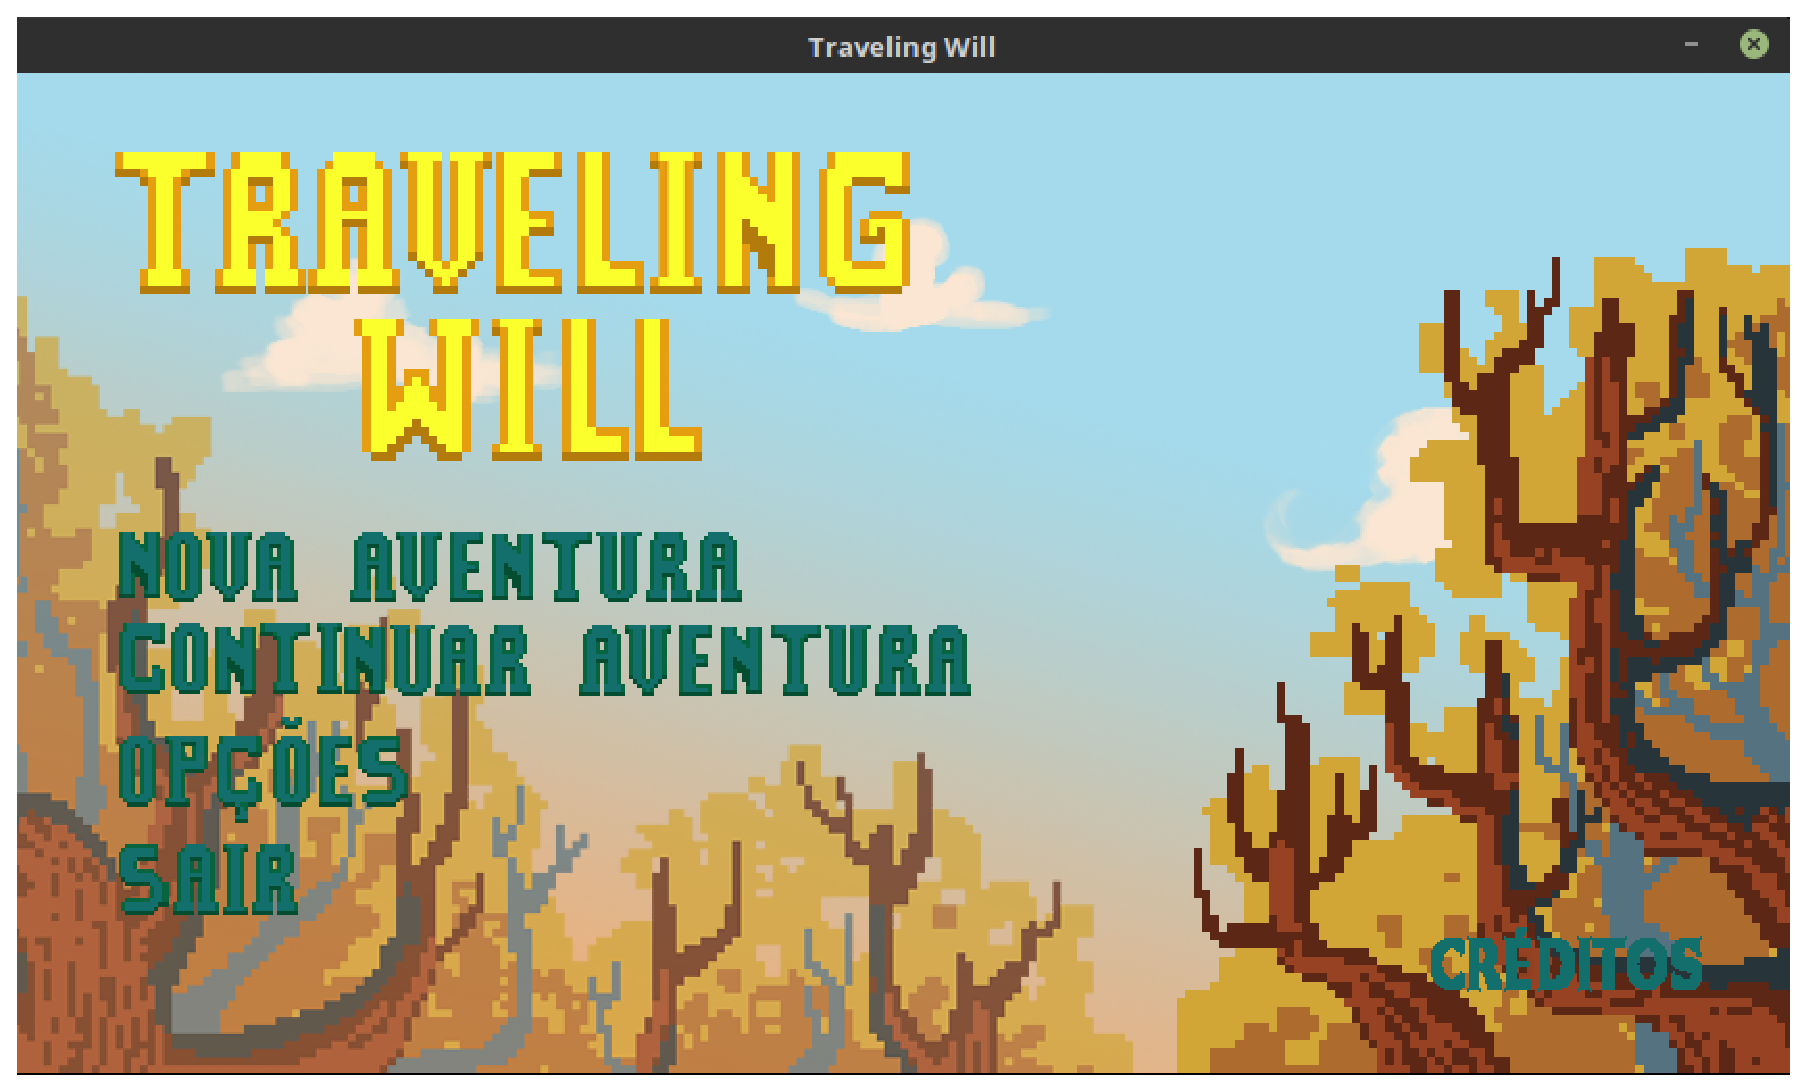
\includegraphics[width=12cm]{figuras/comparacao/pc-menu.eps} }}%
    \qquad
    \subfloat[Menu portado. Fonte: \textit{Autores}.]{{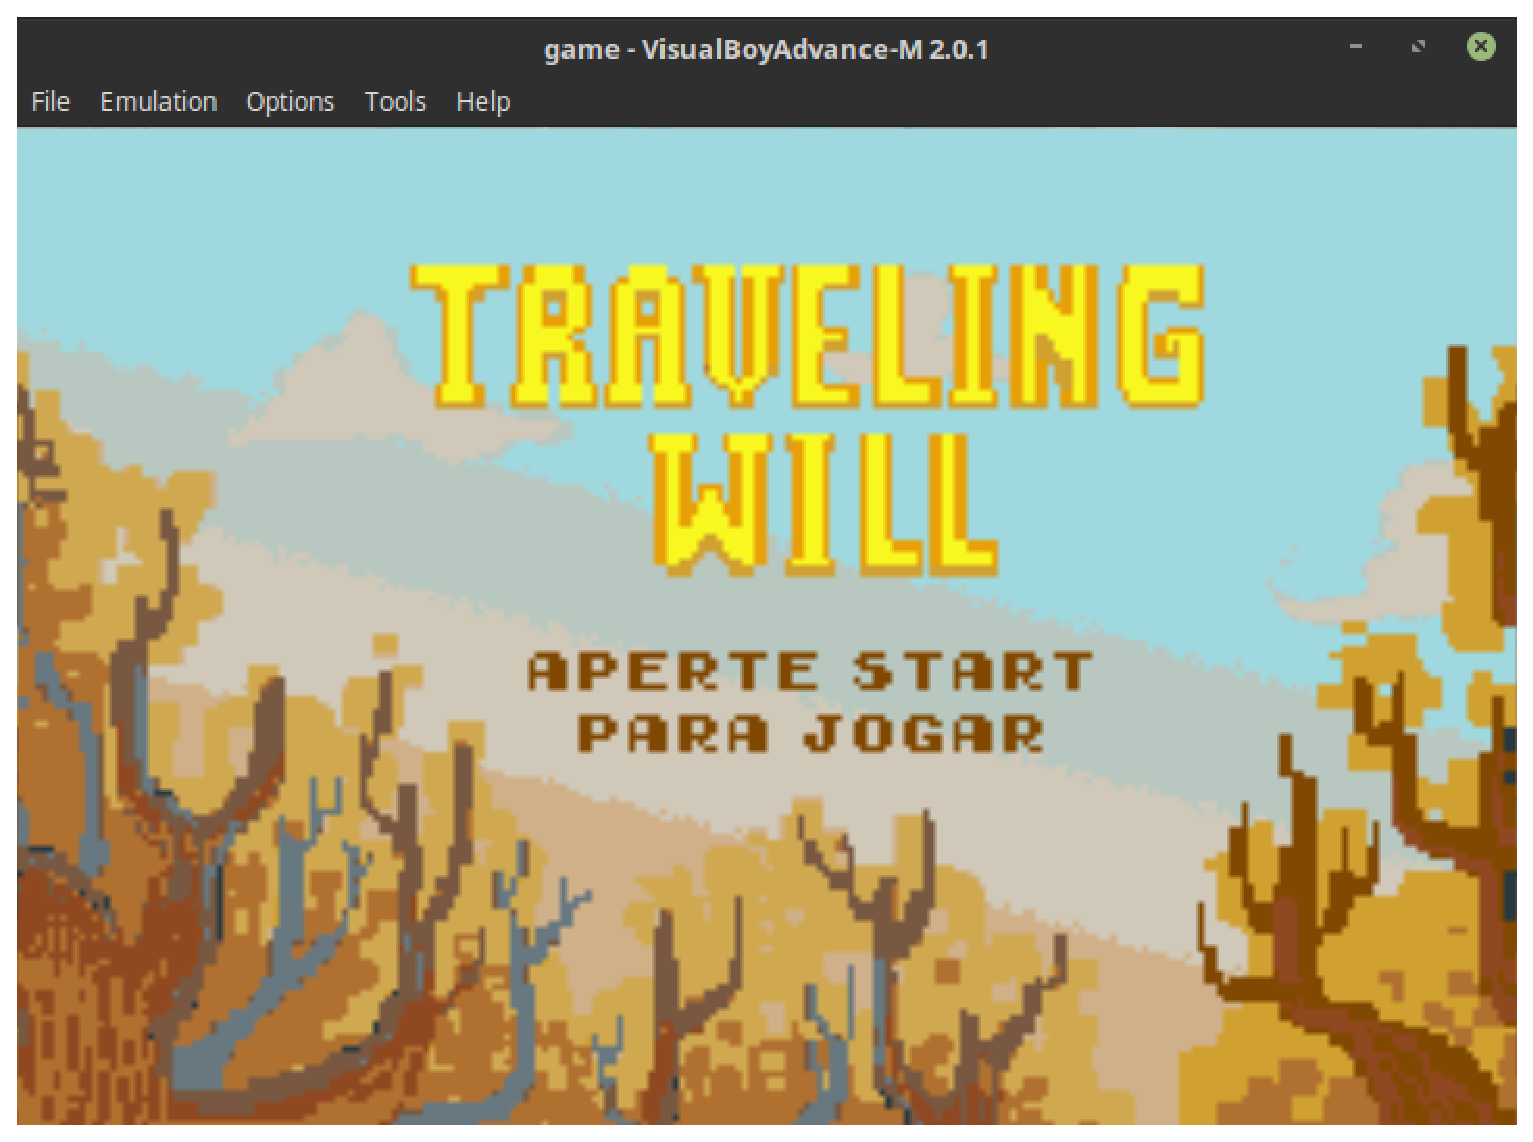
\includegraphics[width=12cm]{figuras/comparacao/gba-menu.eps} }}%
    \caption{Comparação do menu principal.}%
    \label{fig:example}%
\end{figure}

\begin{figure}%
    \centering
    \subfloat[Primeira fase original. Fonte: \textit{Autores}.]{{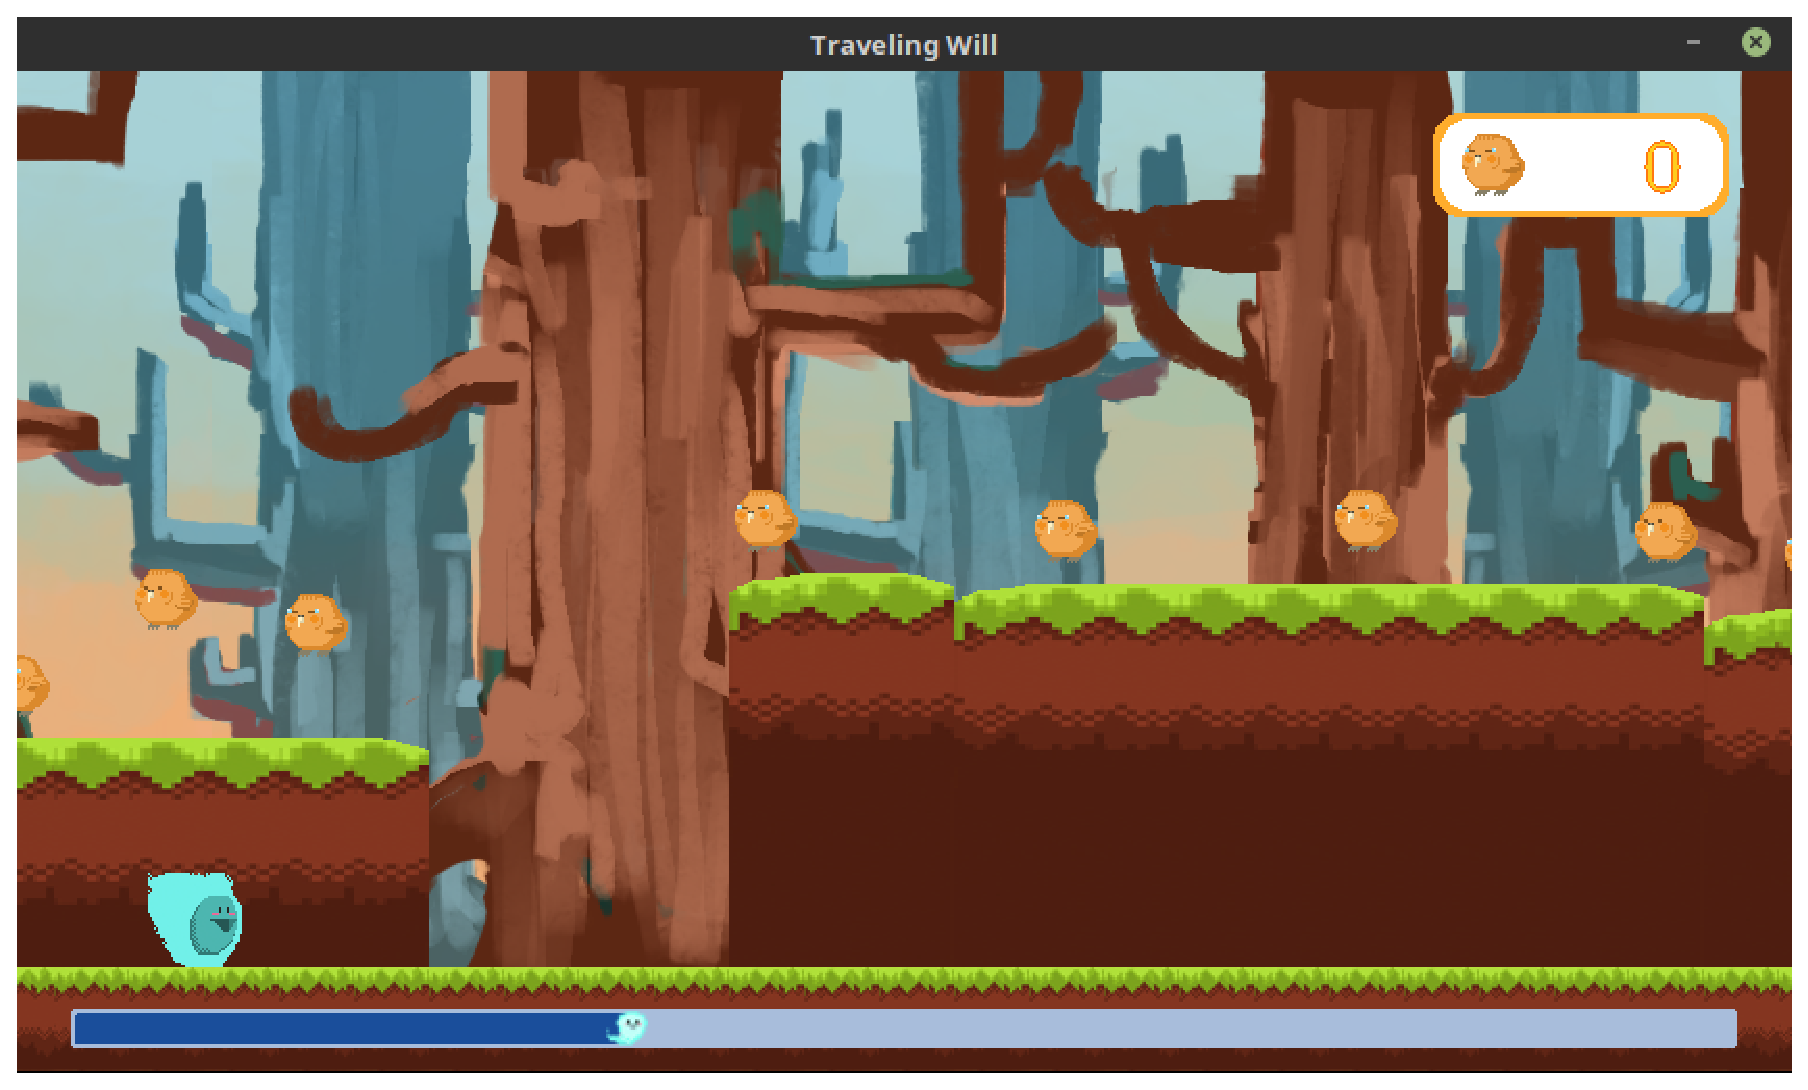
\includegraphics[width=12cm]{figuras/comparacao/pc-fase1.eps} }}%
    \qquad
    \subfloat[Primeira fase portada. Fonte: \textit{Autores}.]{{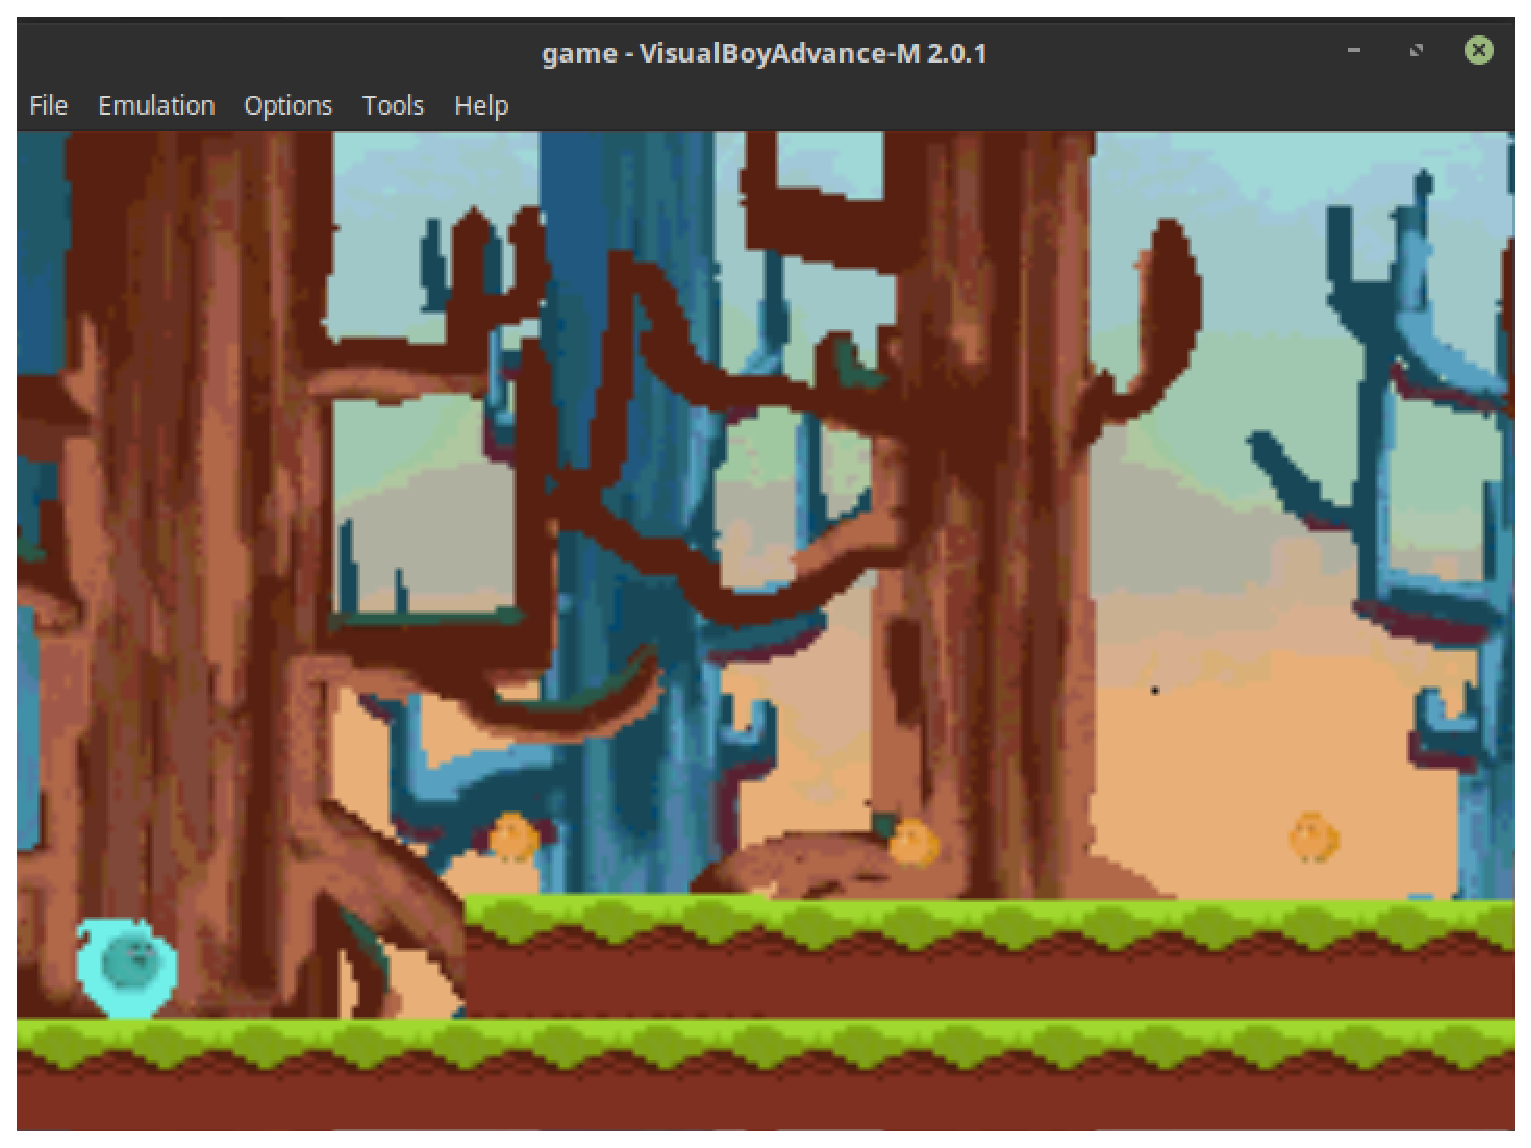
\includegraphics[width=12cm]{figuras/comparacao/gba-fase1.eps} }}%
    \caption{Comparação da primeira fase.}%
    \label{fig:example}%
\end{figure}

\begin{figure}%
    \centering
    \subfloat[Segunda fase original. Fonte: \textit{Autores}.]{{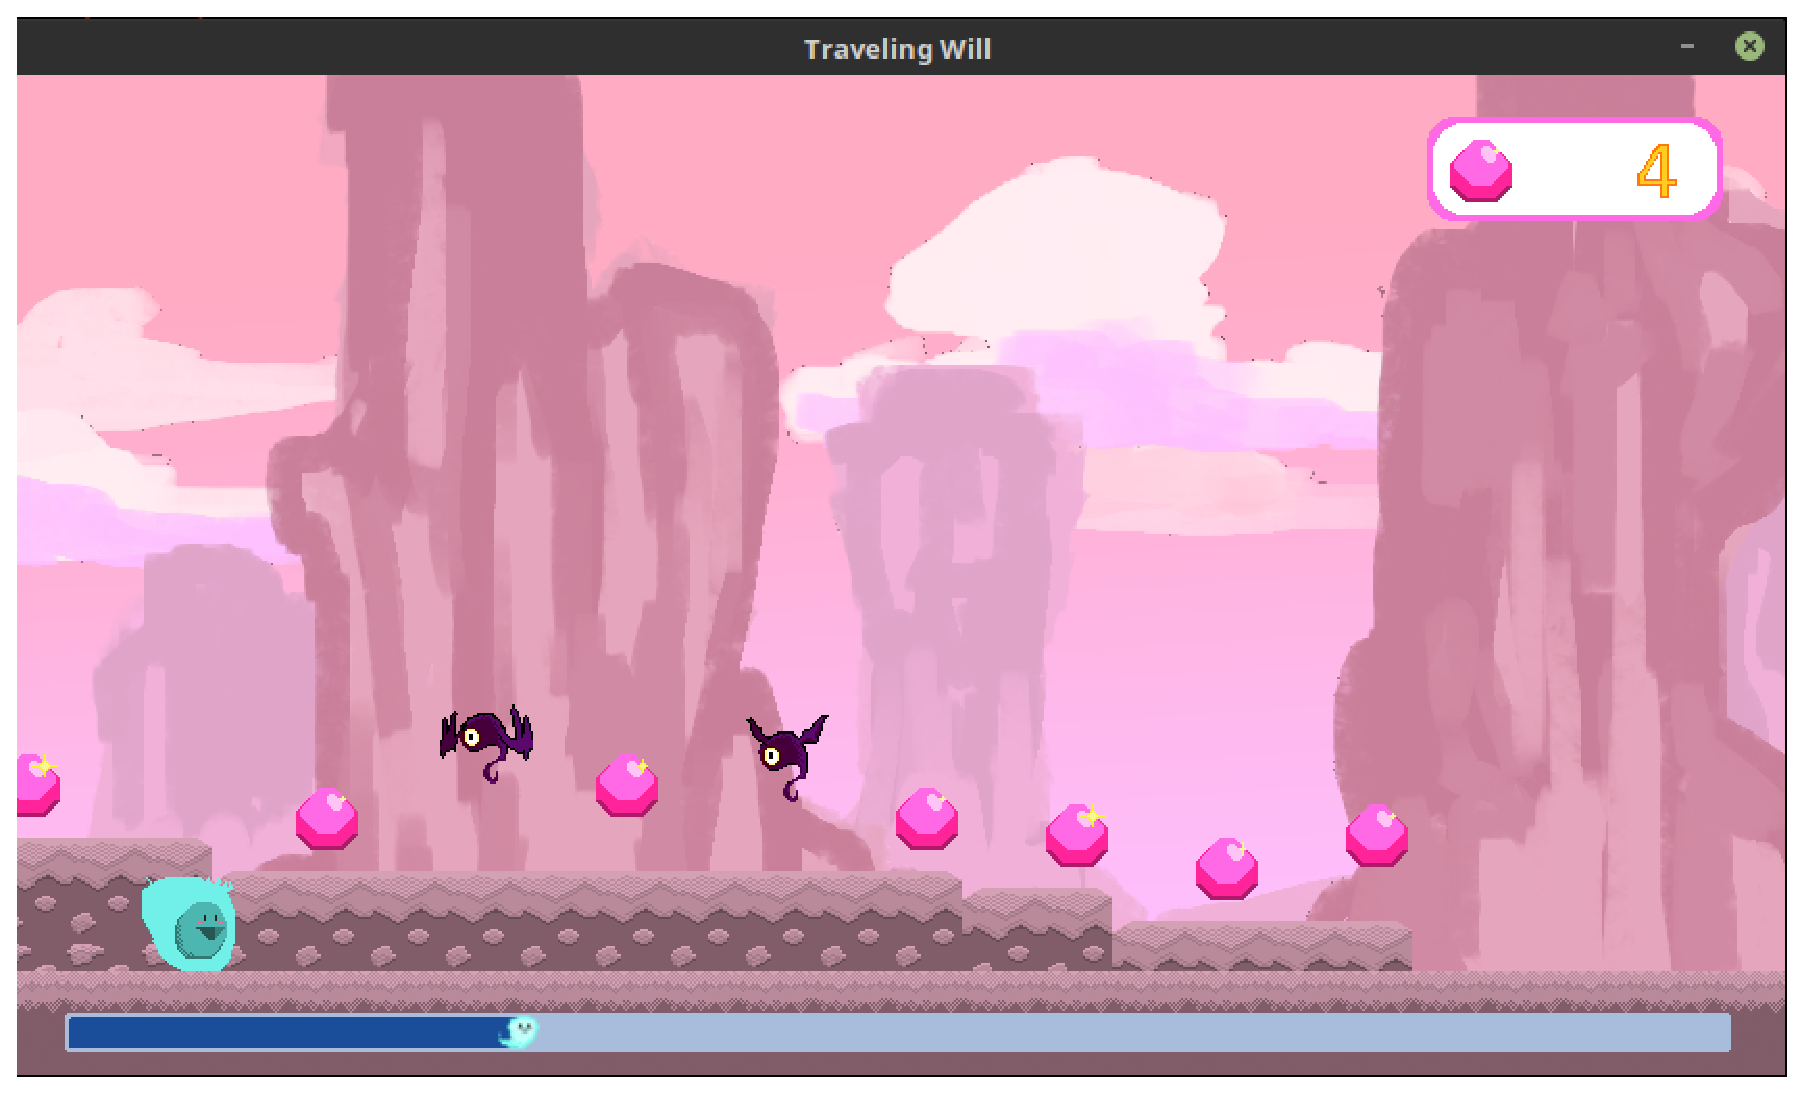
\includegraphics[width=12cm]{figuras/comparacao/pc-fase2.eps} }}%
    \qquad
    \subfloat[Segunda fase portada. Fonte: \textit{Autores}.]{{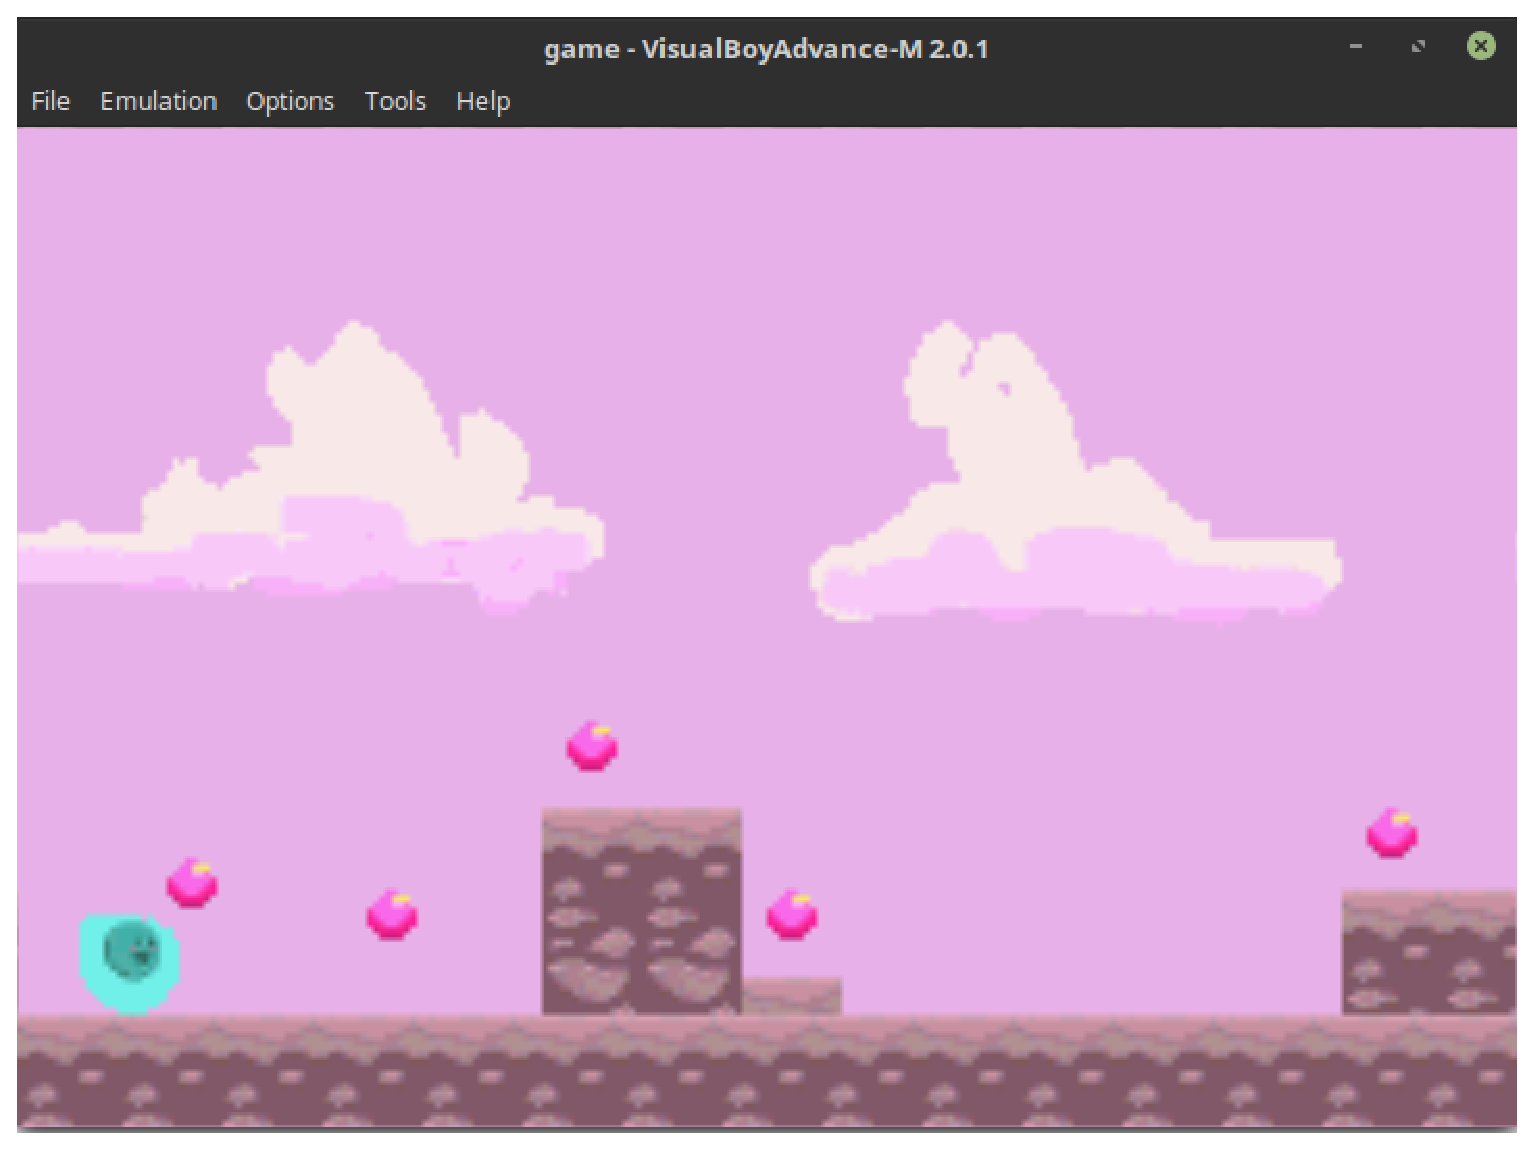
\includegraphics[width=12cm]{figuras/comparacao/gba-fase2.eps} }}%
    \caption{Comparação da segunda fase.}%
    \label{fig:example}%
\end{figure}

\begin{figure}%
    \centering
    \subfloat[Terceira fase original. Fonte: \textit{Autores}.]{{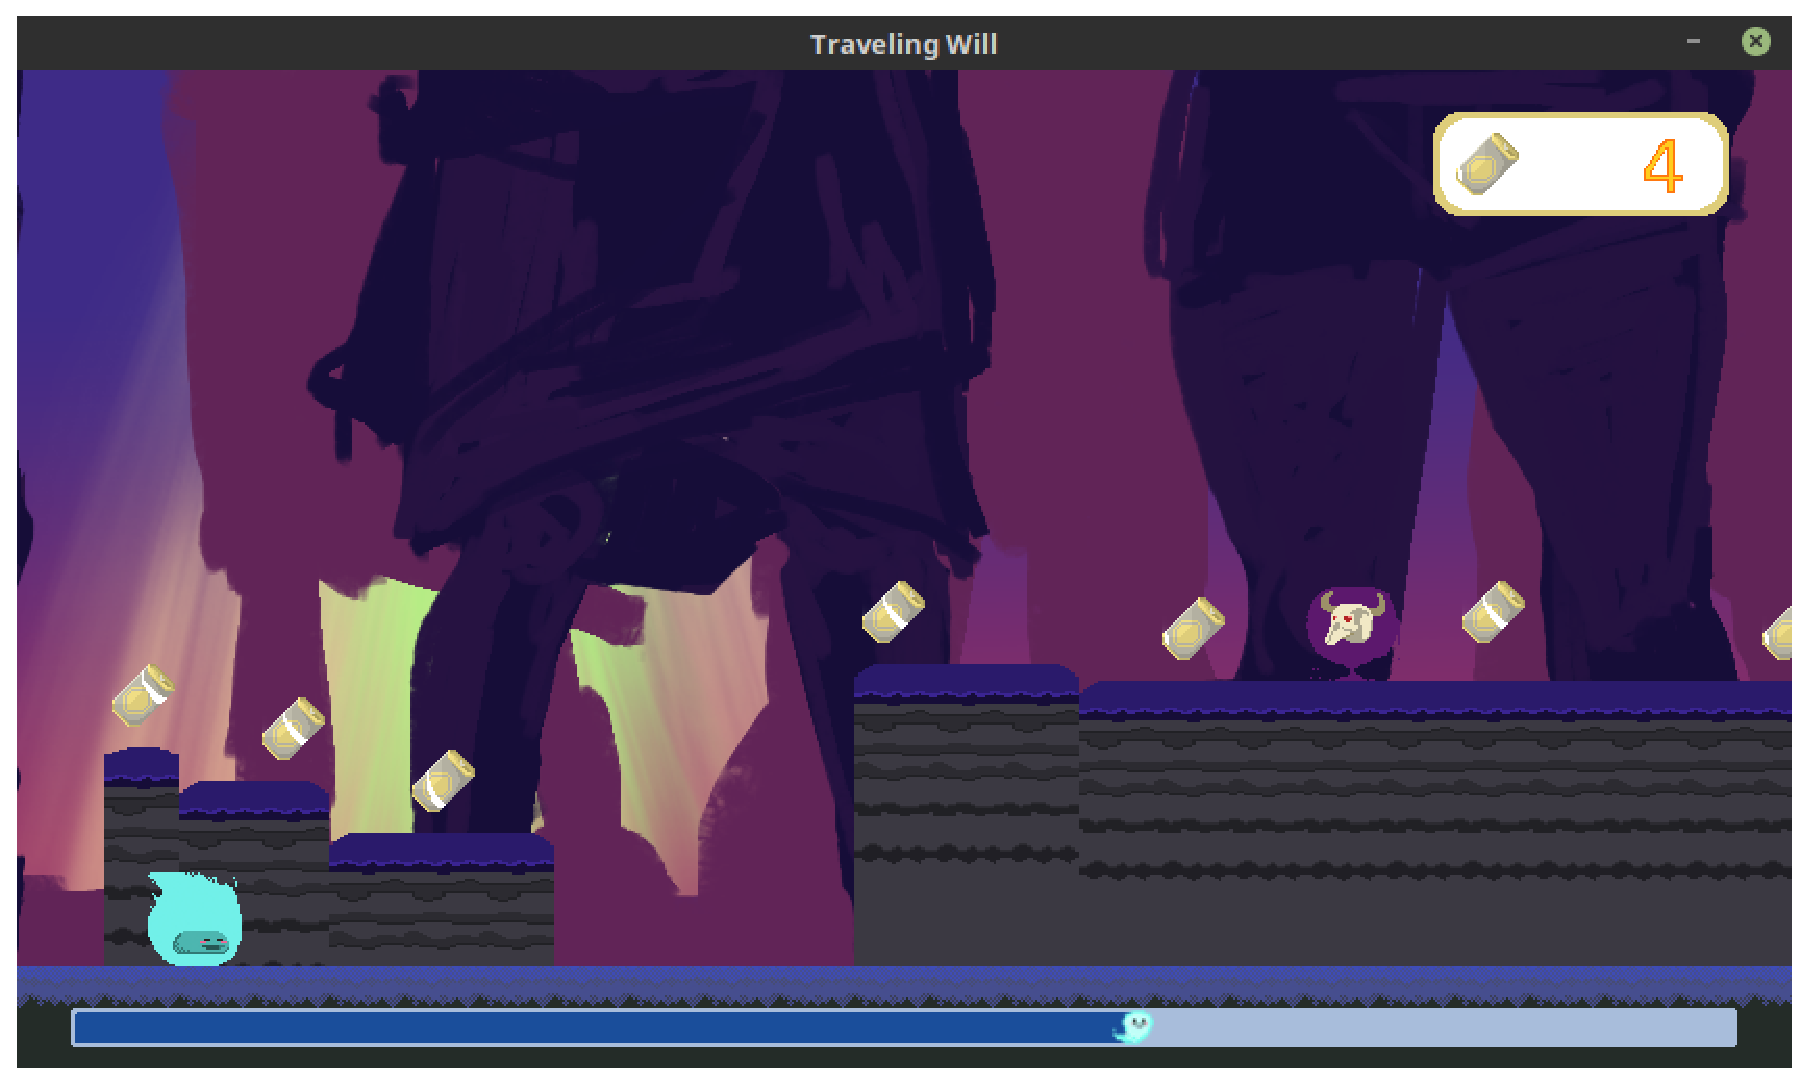
\includegraphics[width=12cm]{figuras/comparacao/pc-fase3.eps} }}%
    \qquad
    \subfloat[Terceira fase portada. Fonte: \textit{Autores}.]{{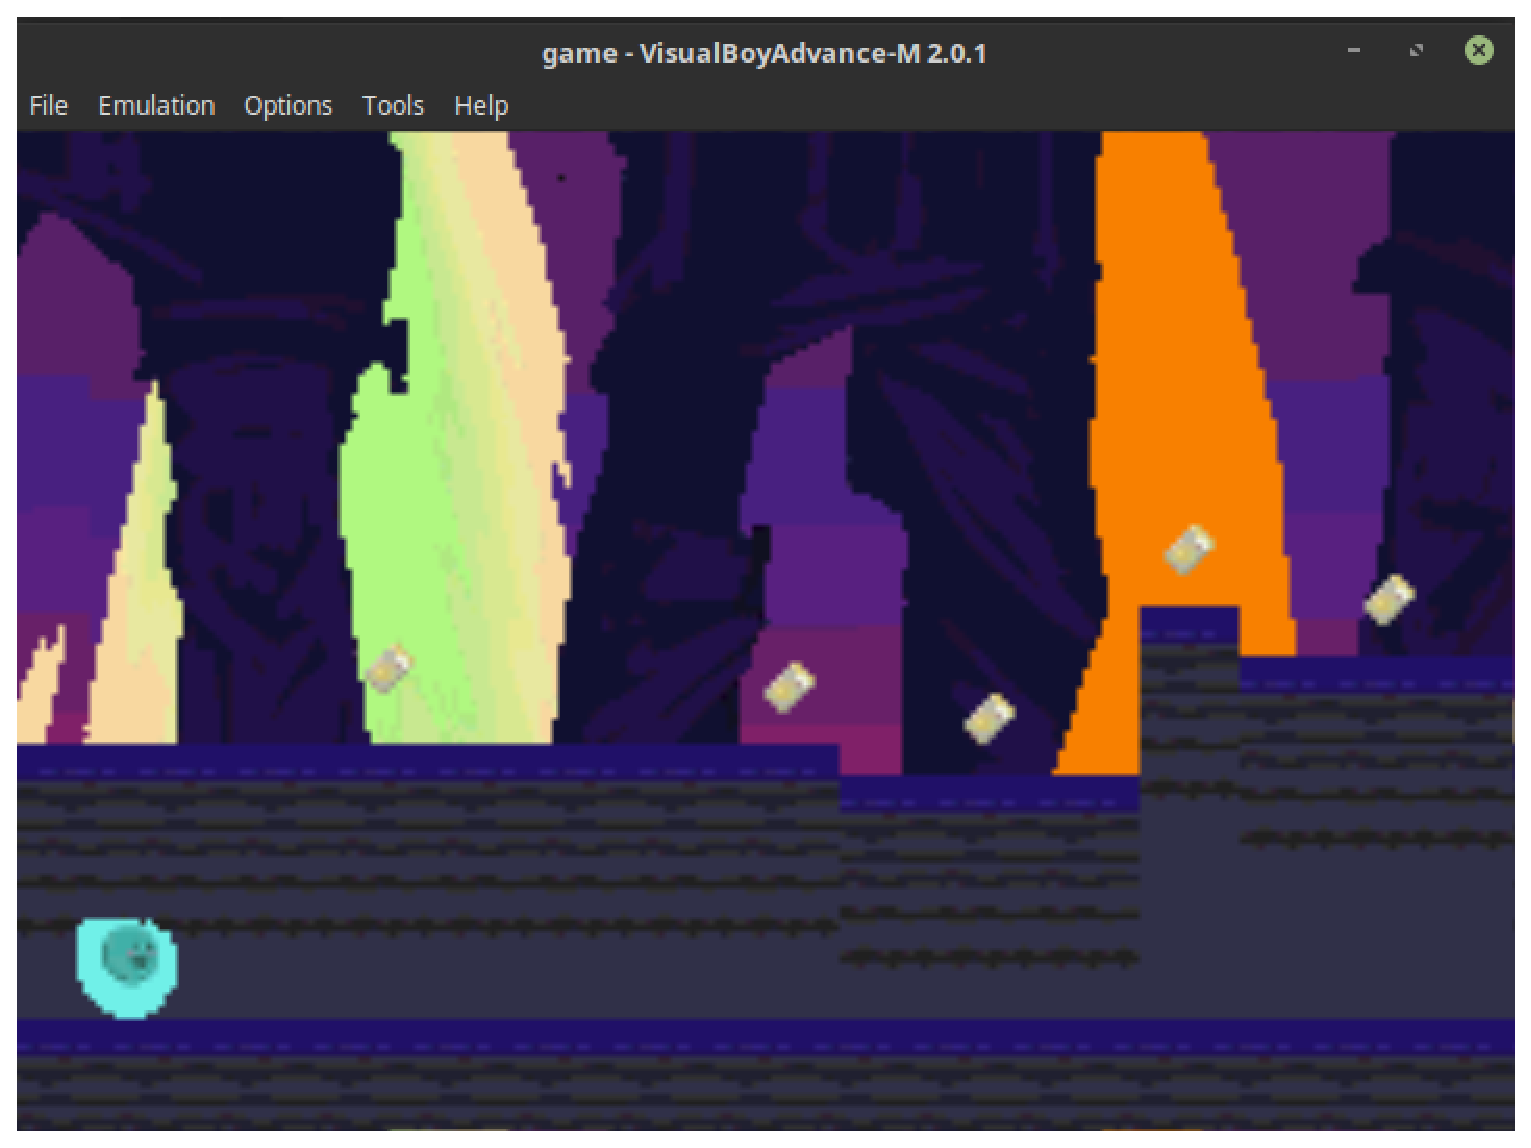
\includegraphics[width=12cm]{figuras/comparacao/gba-fase3.eps} }}%
    \caption{Comparação da terceira fase.}%
    \label{fig:example}%
\end{figure}

\begin{figure}%
    \centering
    \subfloat[Quarta fase original. Fonte: \textit{Autores}.]{{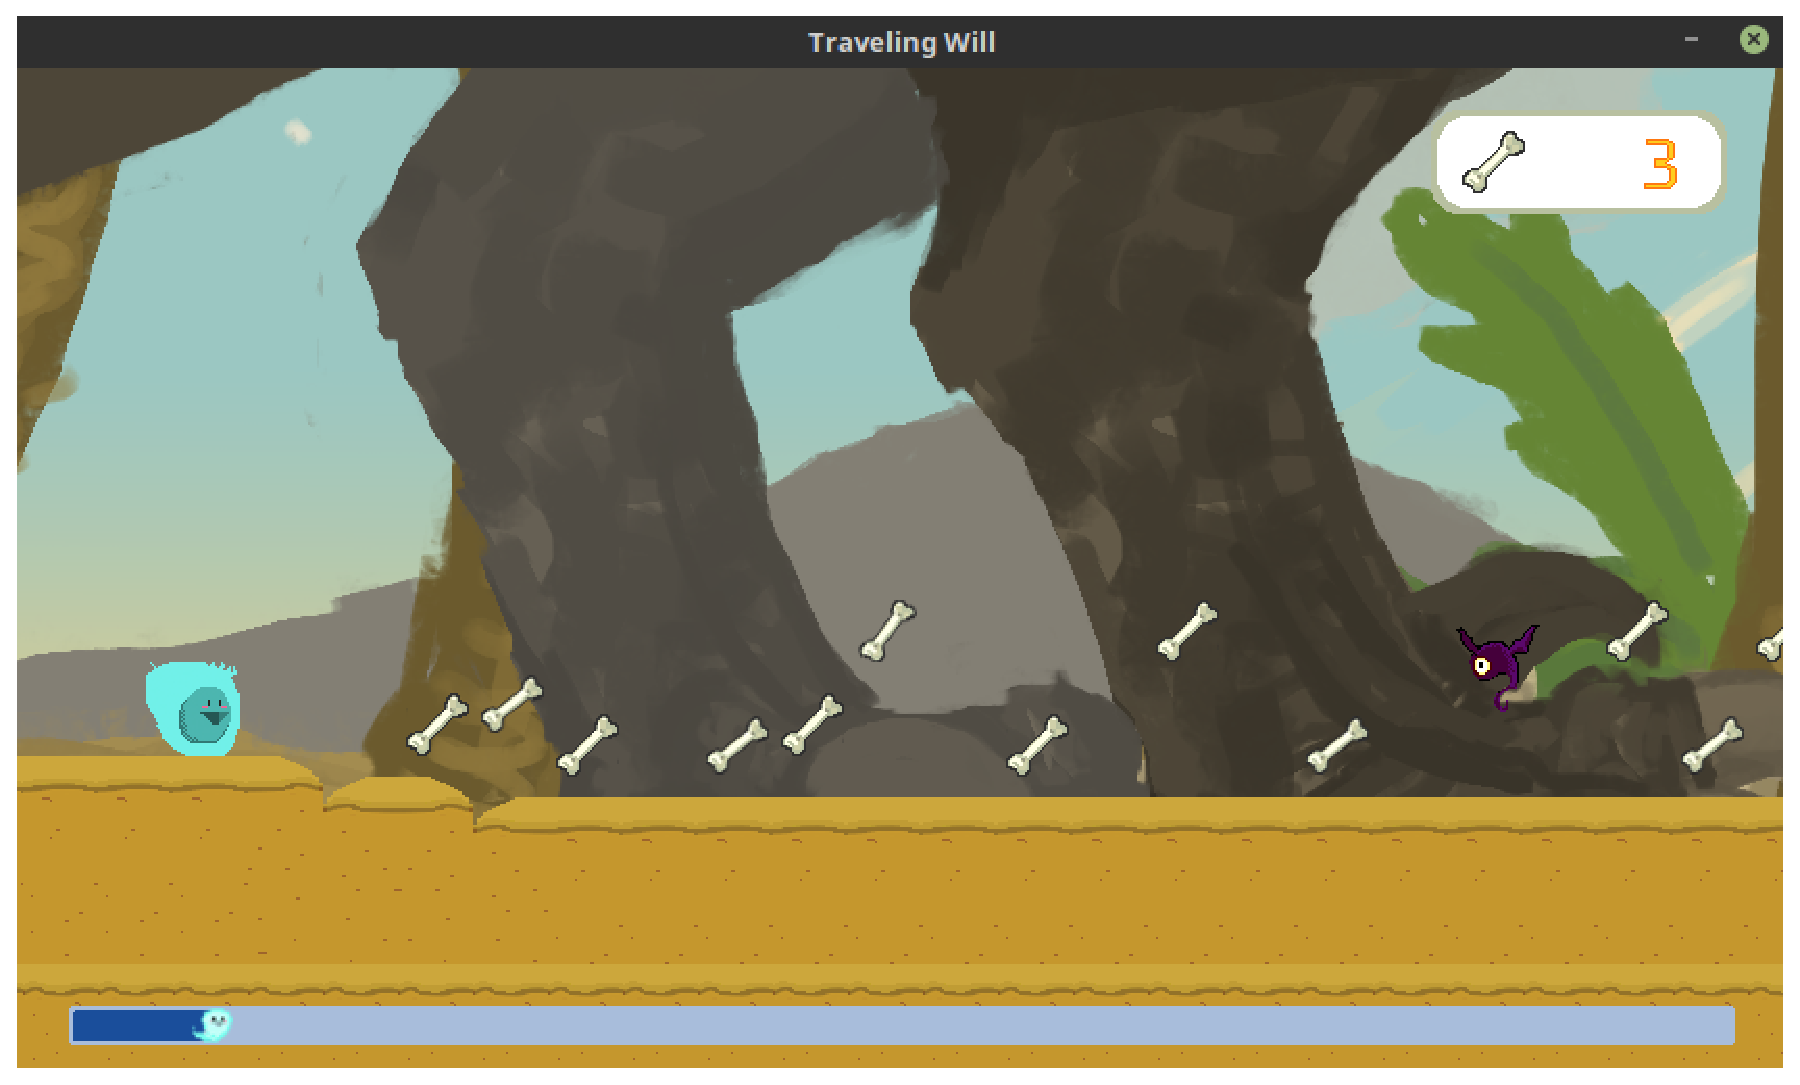
\includegraphics[width=12cm]{figuras/comparacao/pc-fase4.eps} }}%
    \qquad
    \subfloat[Quarta fase portada. Fonte: \textit{Autores}.]{{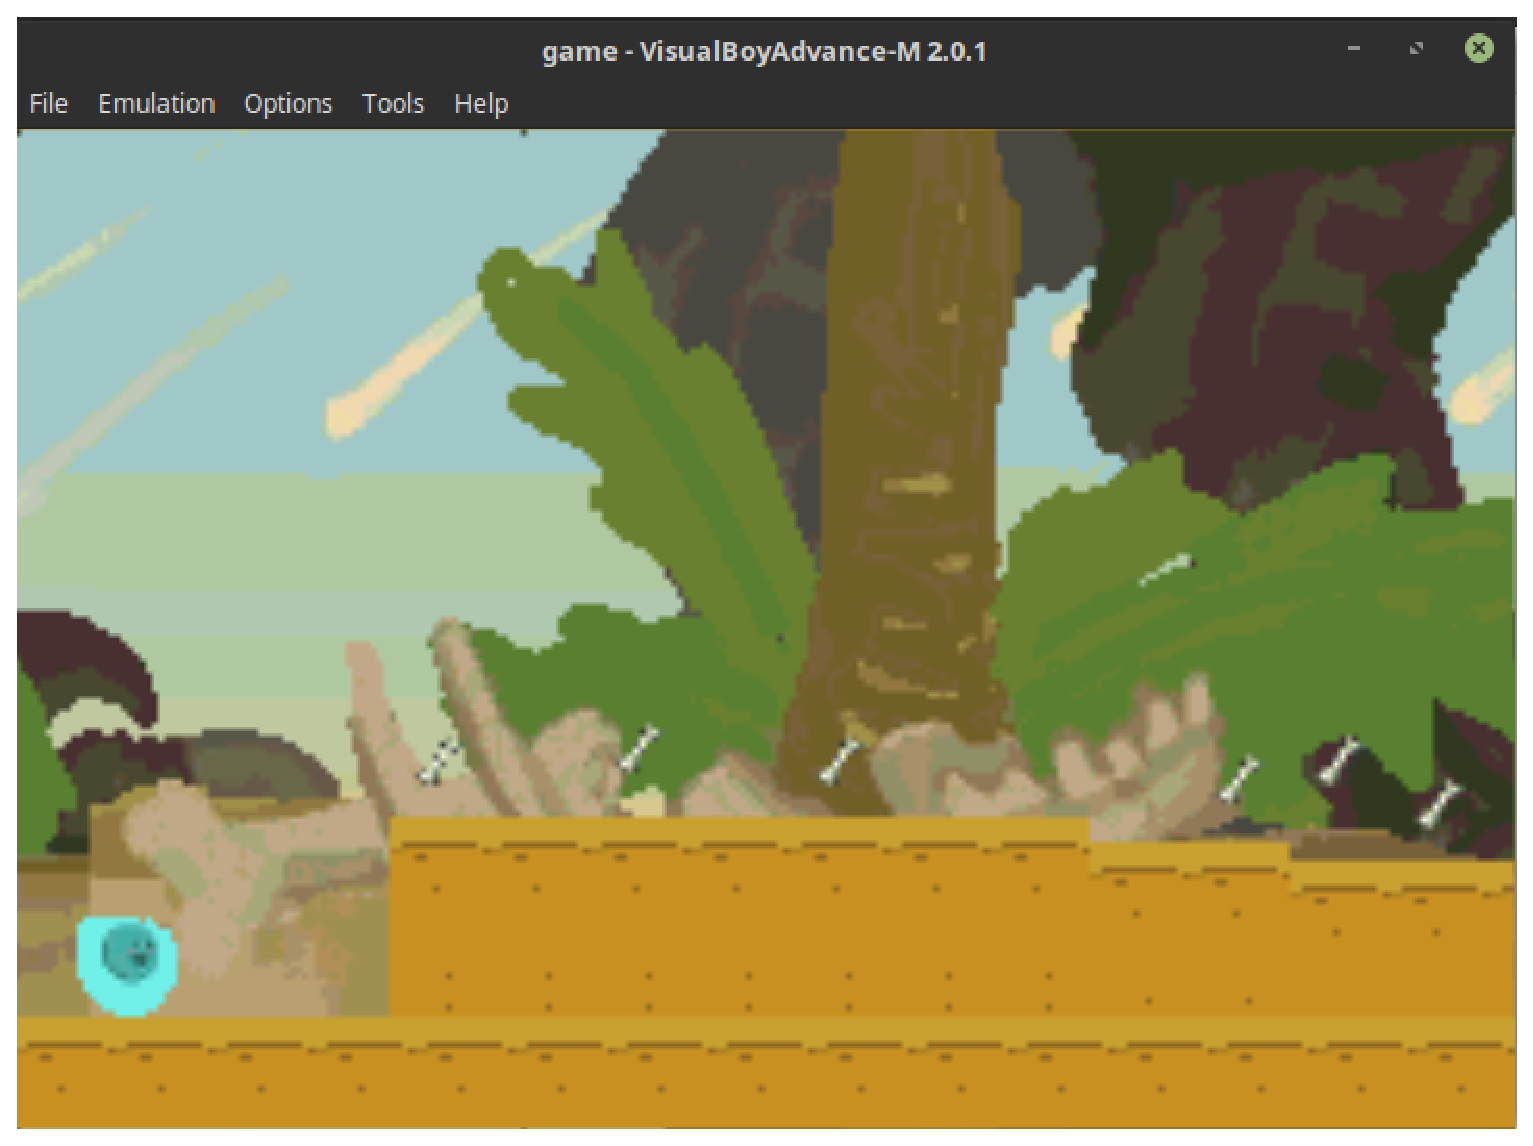
\includegraphics[width=12cm]{figuras/comparacao/gba-fase4.eps} }}%
    \caption{Comparação da quarta fase.}%
    \label{fig:example}%
\end{figure}

\begin{figure}%
    \centering
    \subfloat[Quinta fase original. Fonte: \textit{Autores}.]{{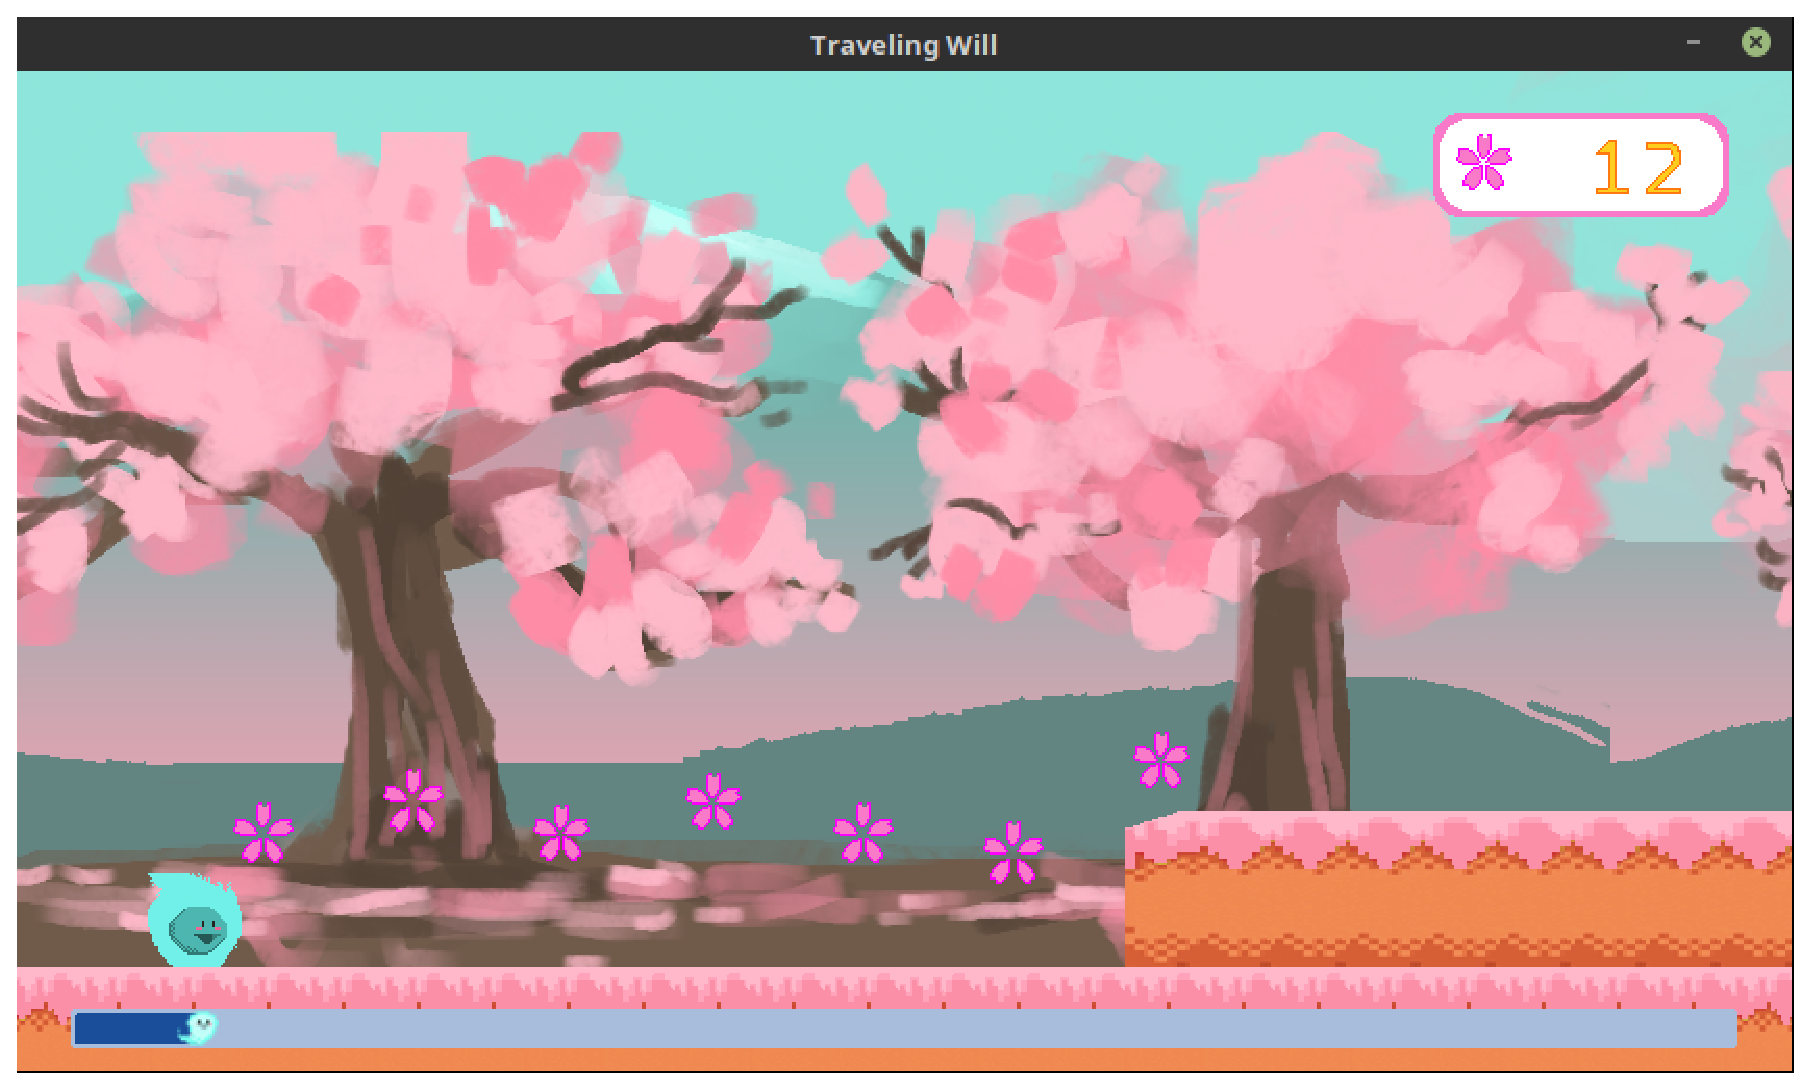
\includegraphics[width=12cm]{figuras/comparacao/pc-fase5.eps} }}%
    \qquad
    \subfloat[Quinta fase portada. Fonte: \textit{Autores}.]{{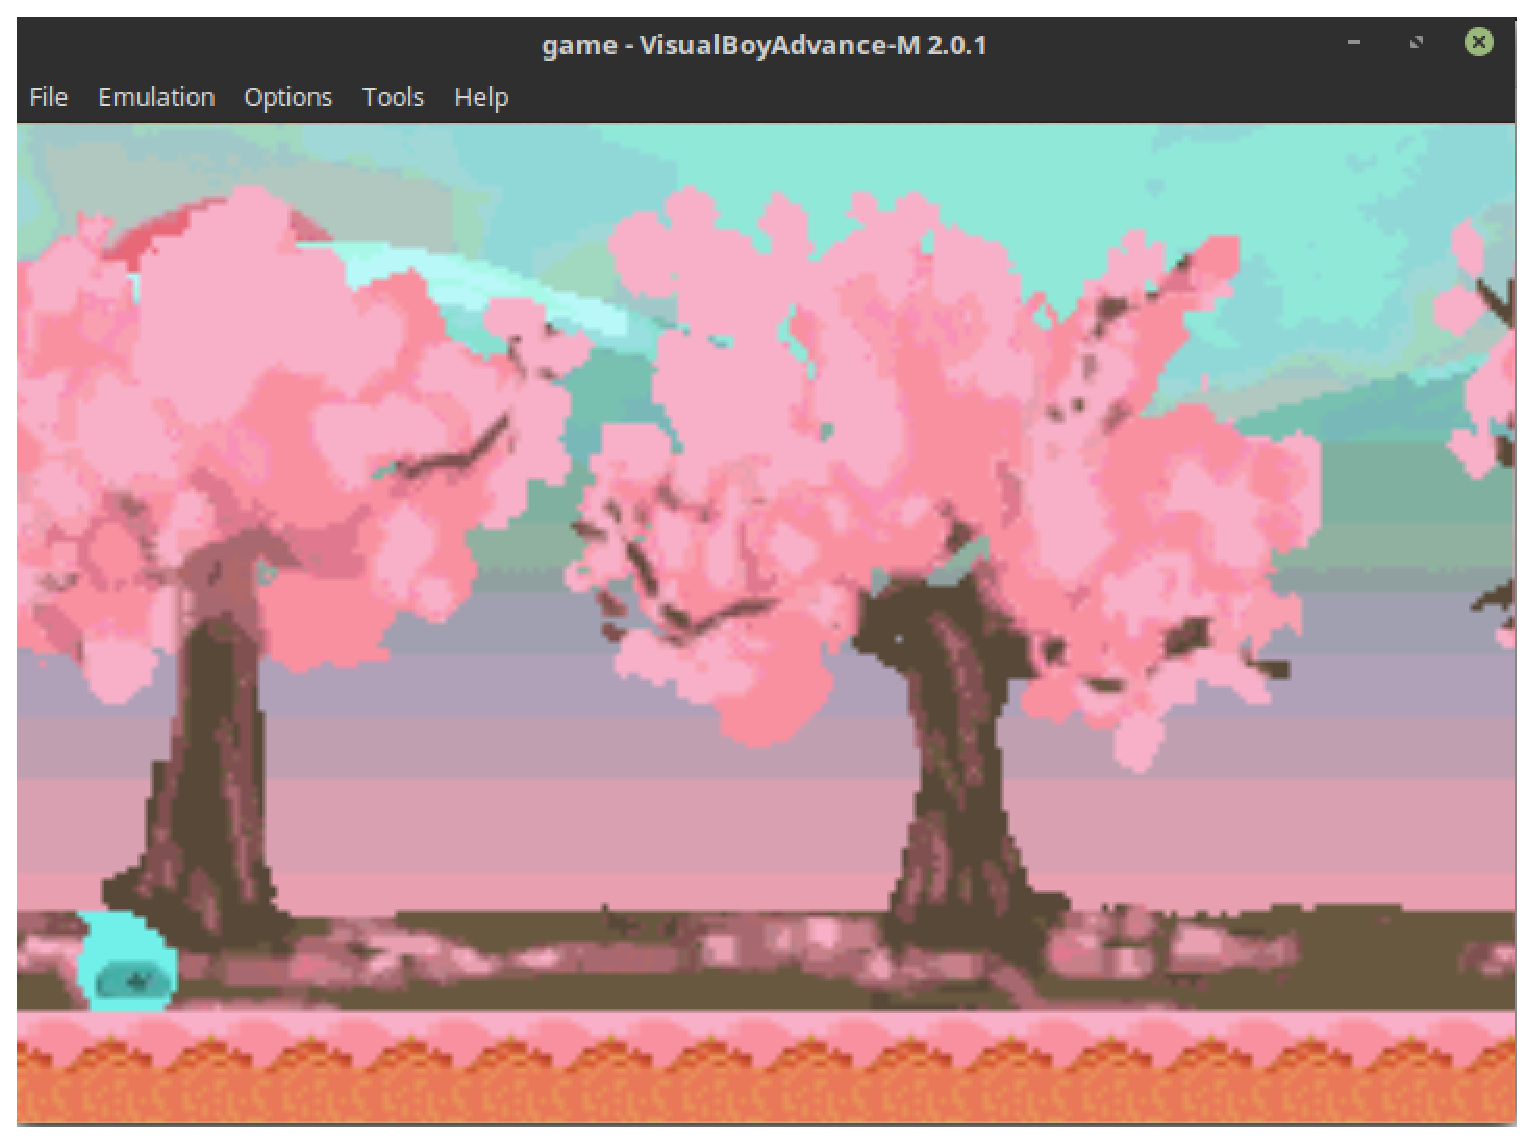
\includegraphics[width=12cm]{figuras/comparacao/gba-fase5.eps} }}%
    \caption{Comparação da quinta fase.}%
    \label{fig:example}%
\end{figure}

\begin{figure}%
    \centering
    \subfloat[Sexta fase original. Fonte: \textit{Autores}.]{{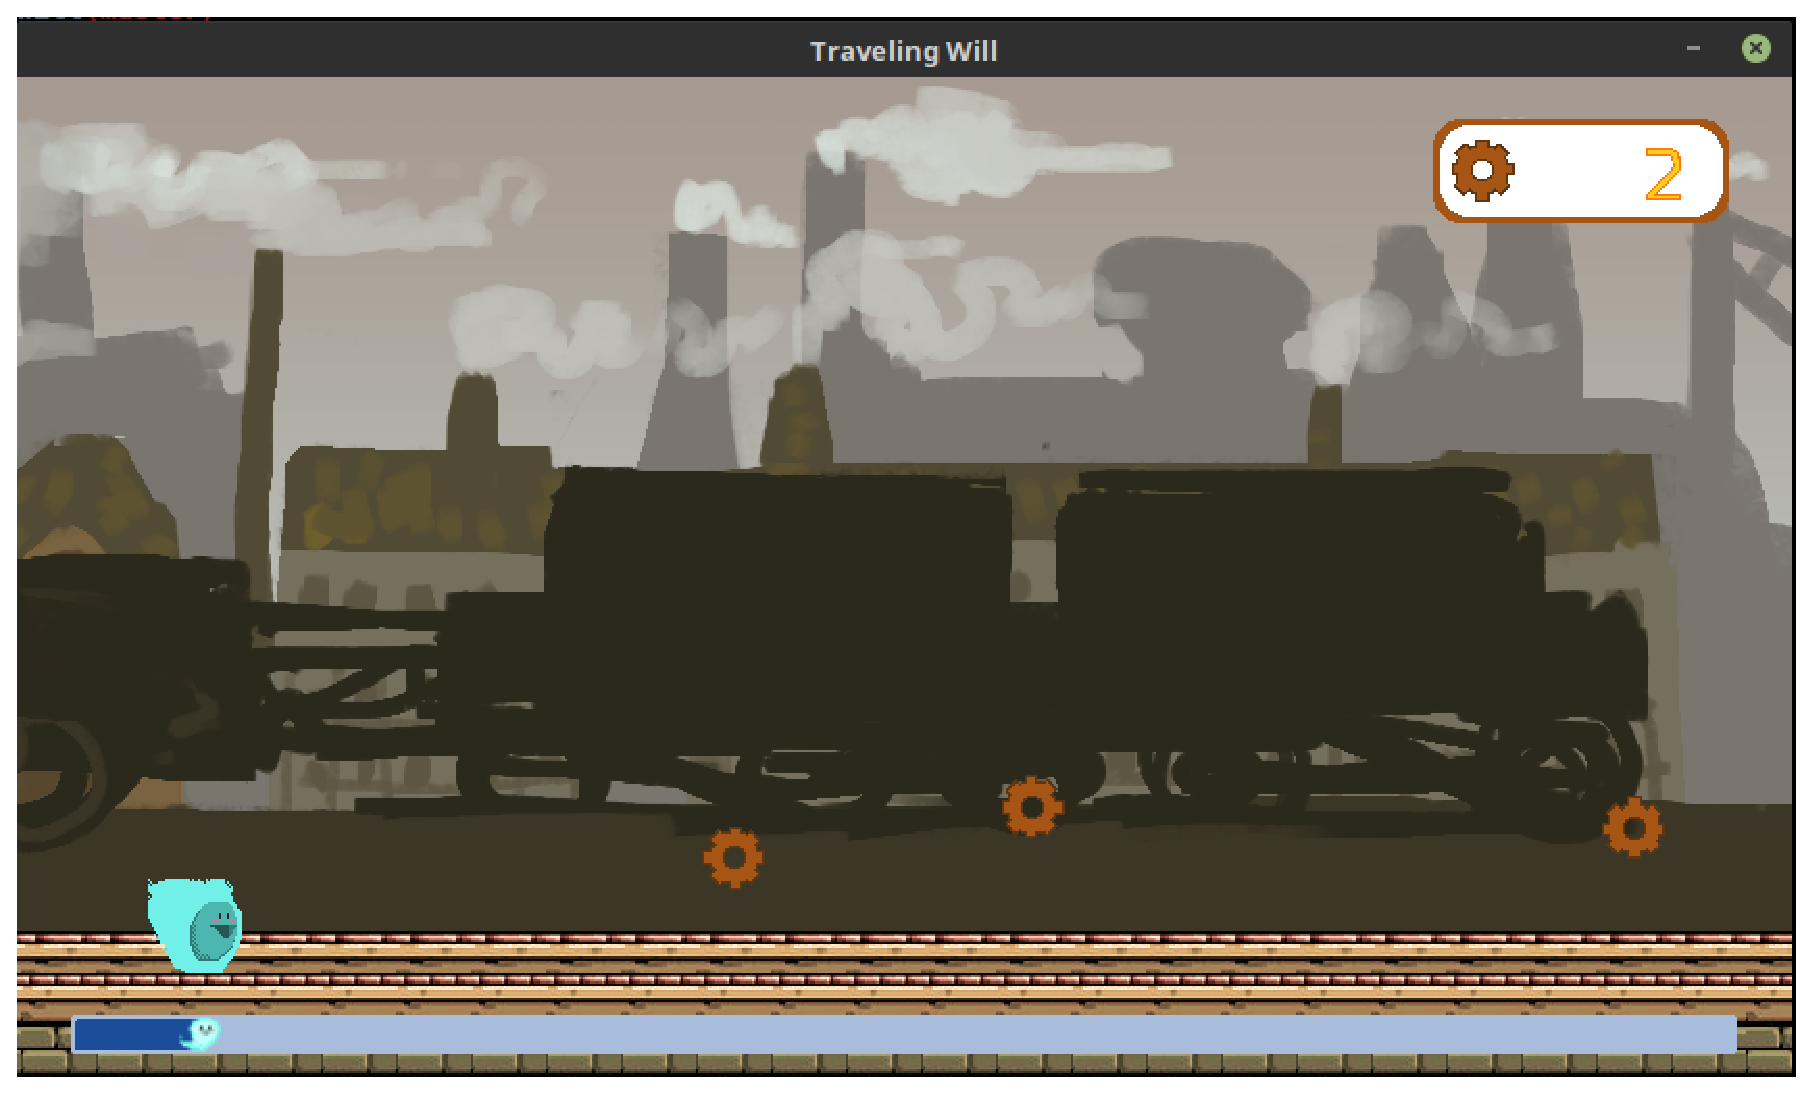
\includegraphics[width=12cm]{figuras/comparacao/pc-fase6.eps} }}%
    \qquad
    \subfloat[Sexta fase portada. Fonte: \textit{Autores}.]{{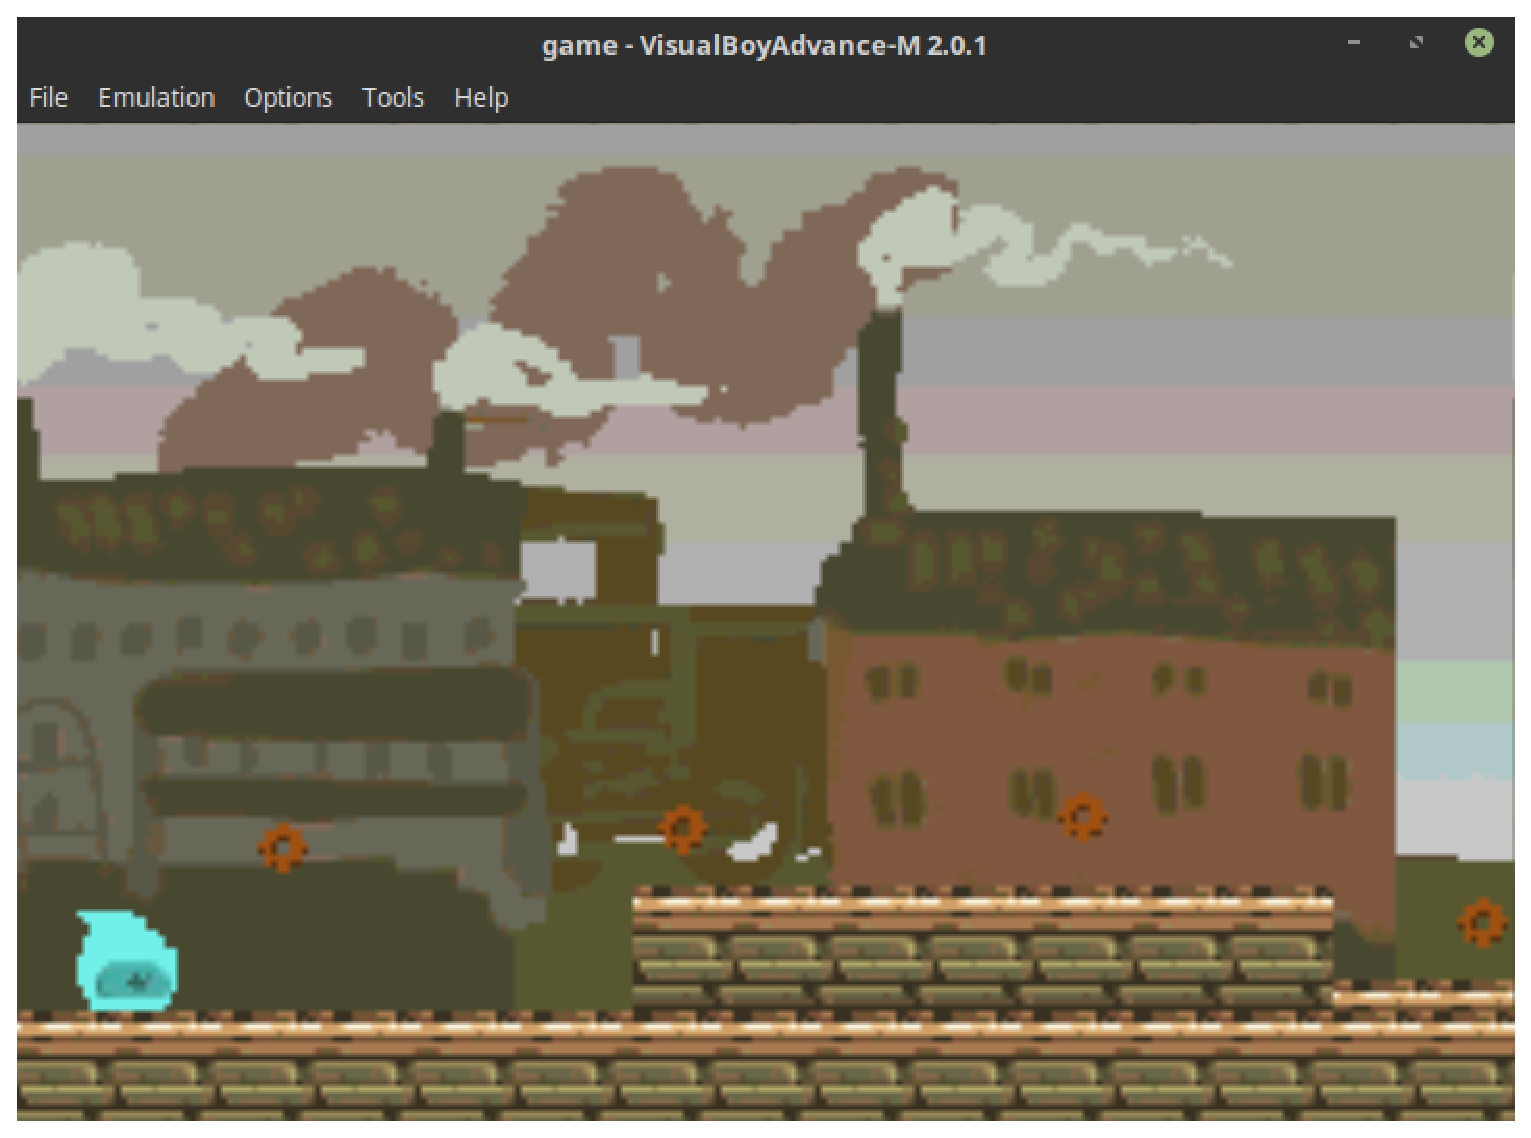
\includegraphics[width=12cm]{figuras/comparacao/gba-fase6.eps} }}%
    \caption{Comparação da sexta fase.}%
    \label{fig:example}%
\end{figure}

\begin{figure}%
    \centering
    \subfloat[Menu de vitória original. Fonte: \textit{Autores}.]{{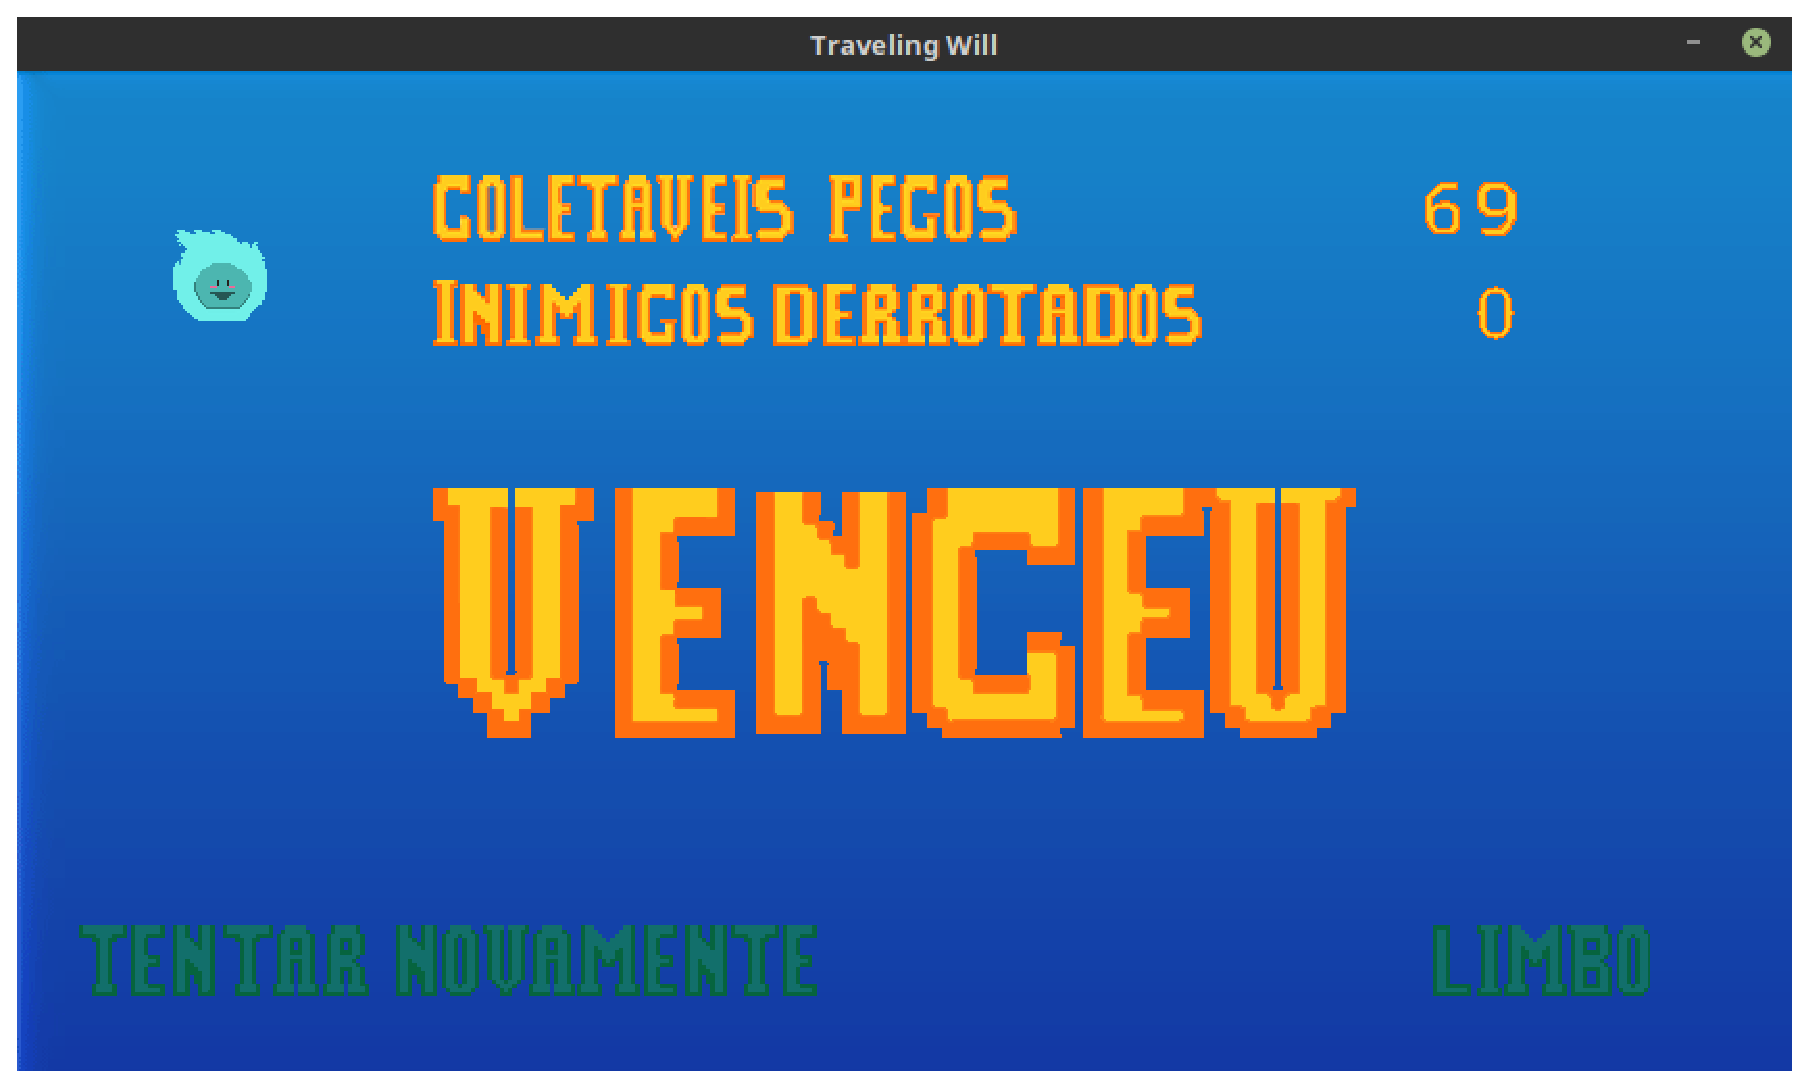
\includegraphics[width=12cm]{figuras/comparacao/pc-vitoria.eps} }}%
    \qquad
    \subfloat[Menu de vitória portado. Fonte: \textit{Autores}.]{{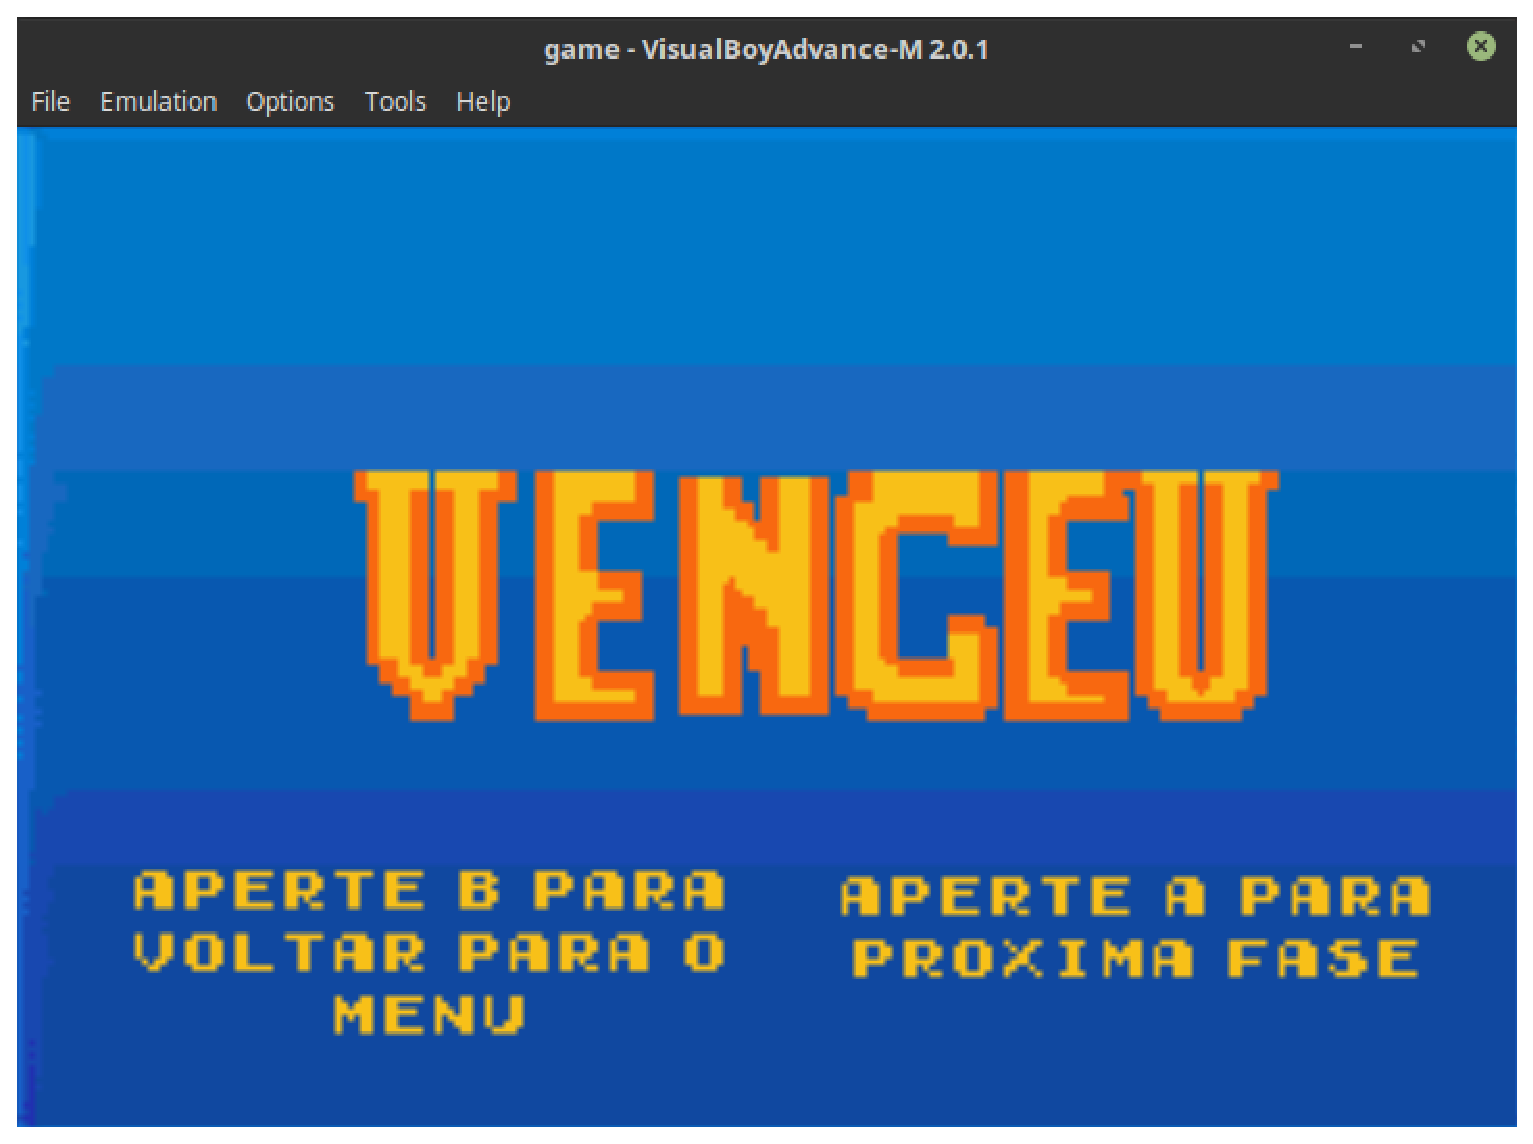
\includegraphics[width=12cm]{figuras/comparacao/gba-vitoria.eps} }}%
    \caption{Comparação do menu de vitória.}%
    \label{fig:example}%
\end{figure}

\begin{figure}%
    \centering
    \subfloat[Menu de derrota original. Fonte: \textit{Autores}.]{{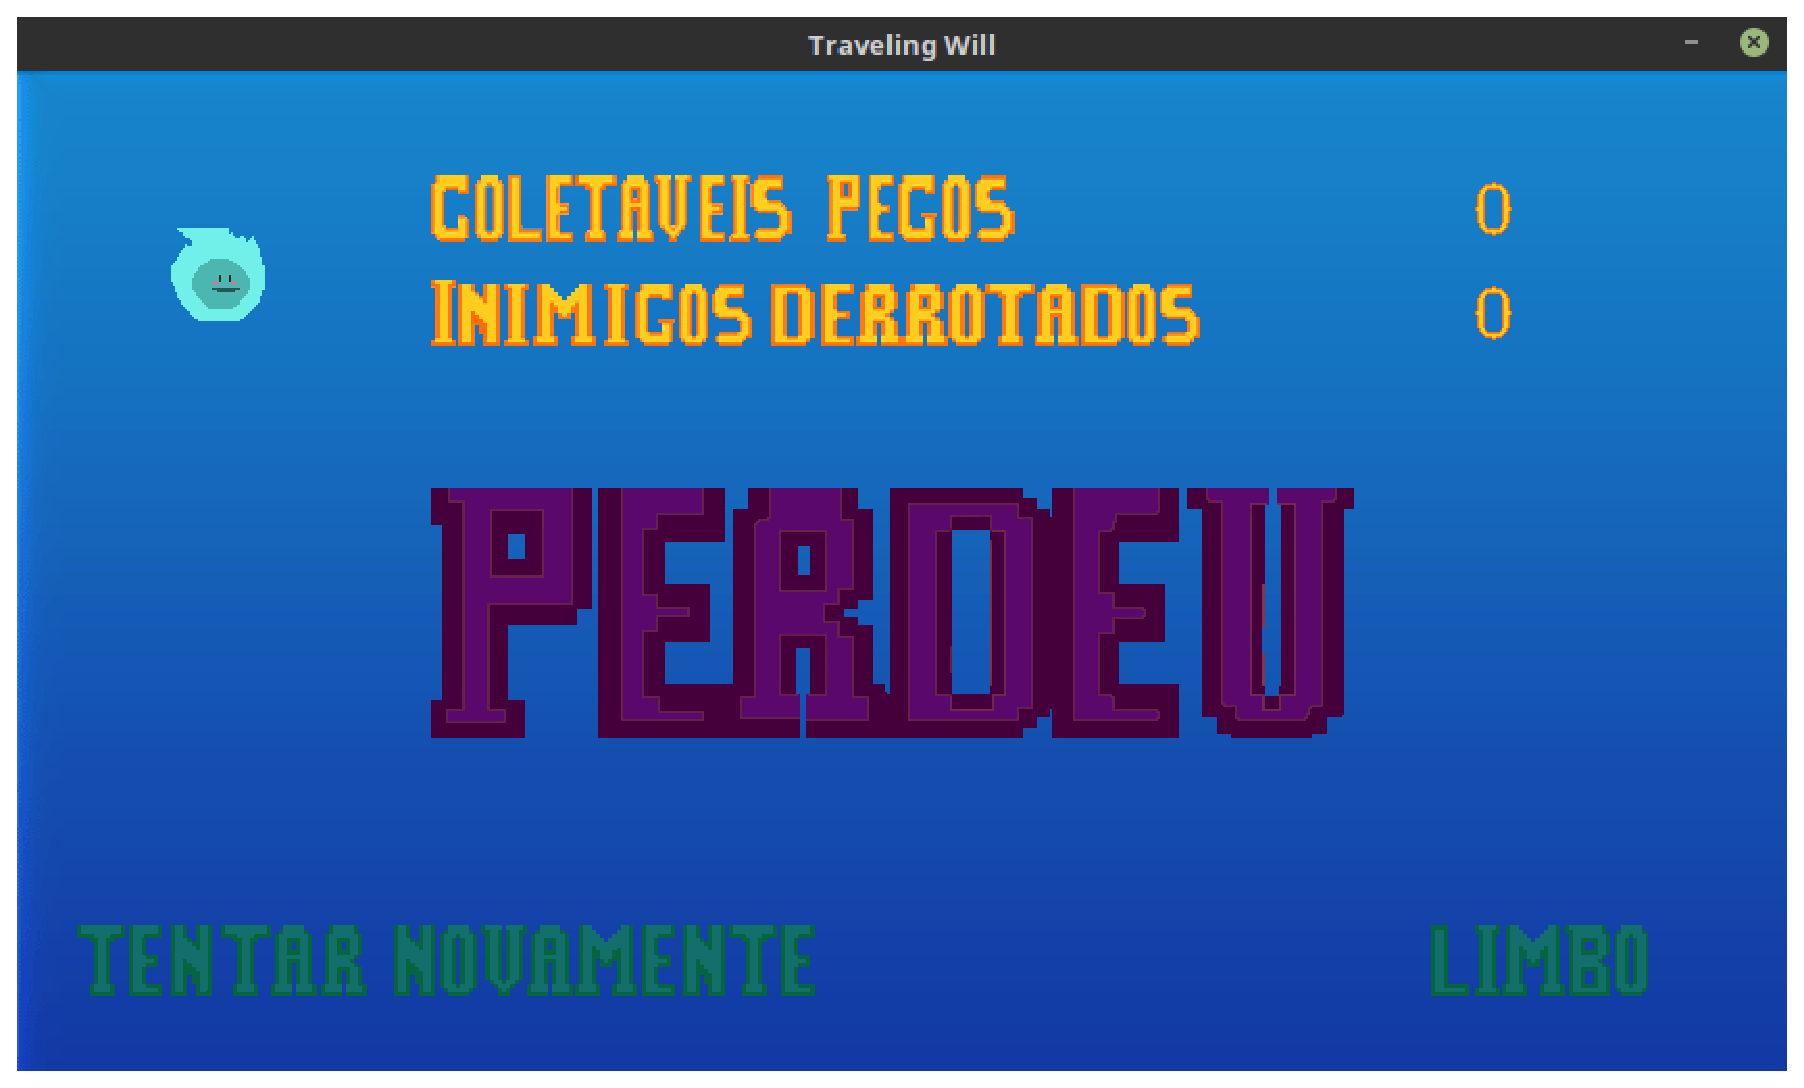
\includegraphics[width=12cm]{figuras/comparacao/pc-defeat.eps} }}%
    \qquad
    \subfloat[Menu de derrota portado. Fonte: \textit{Autores}.]{{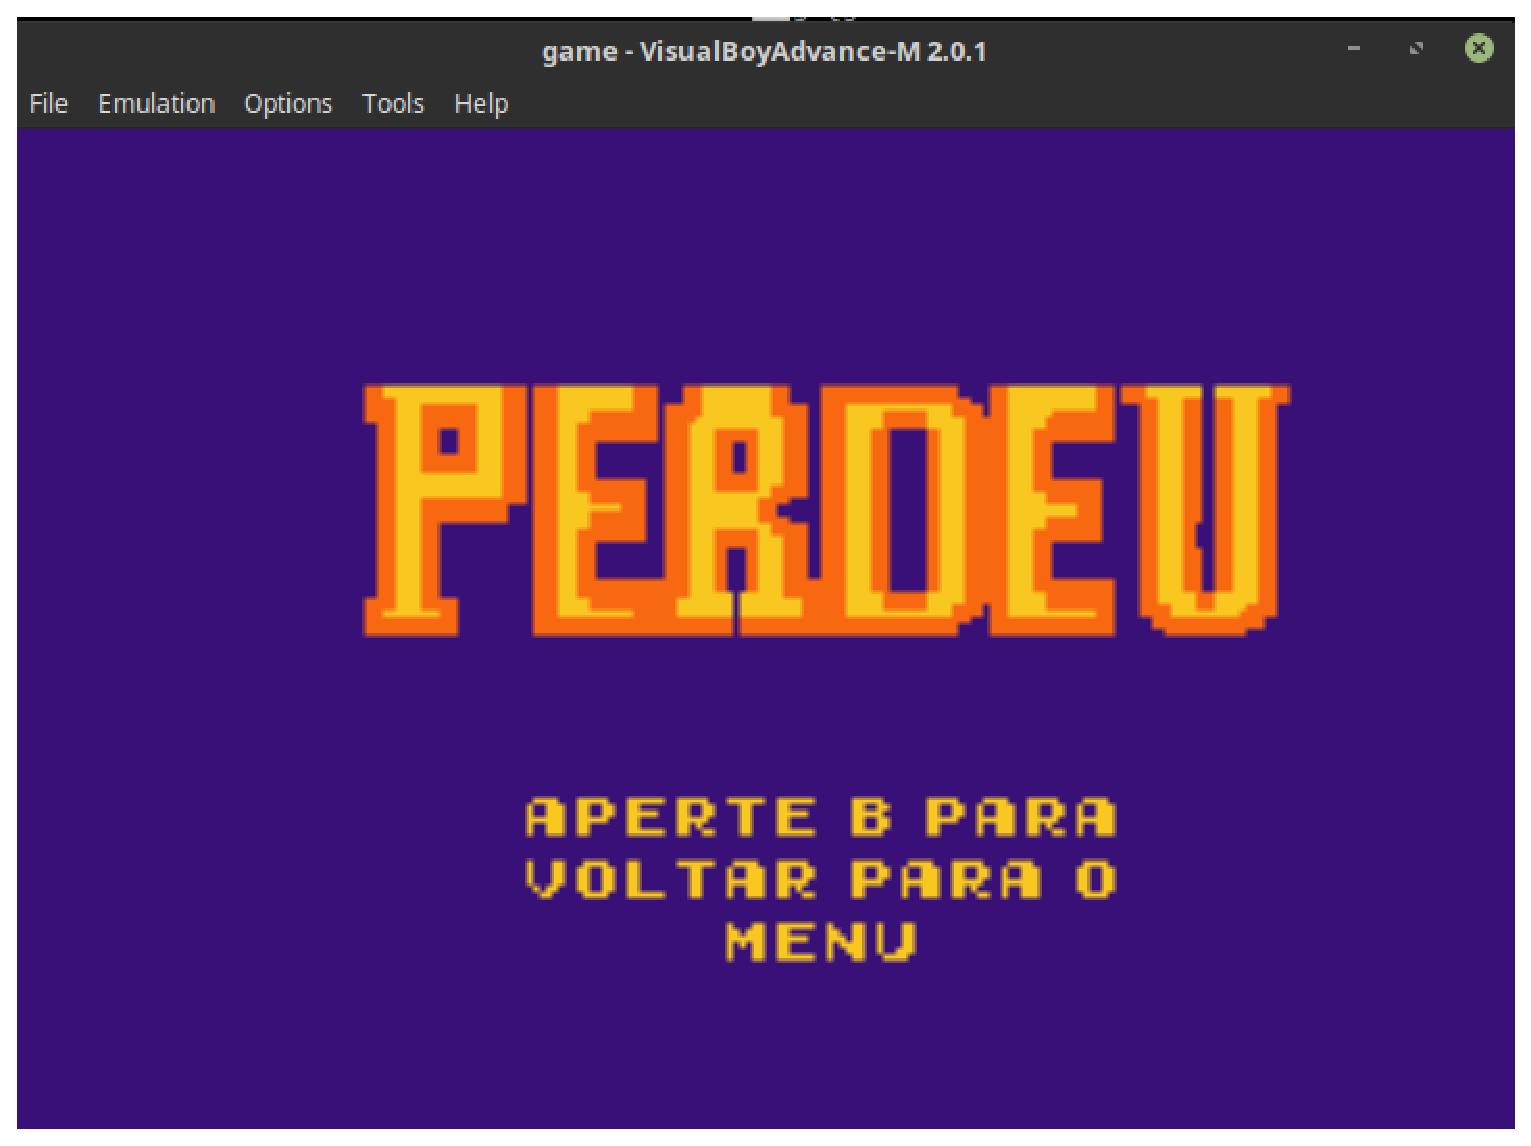
\includegraphics[width=12cm]{figuras/comparacao/gba-defeat.eps} }}%
    \caption{Comparação do menu de derrota.}%
    \label{fig:example}%
\end{figure}

% \begin{figure}%
%     \centering
%     \subfloat[Jogo original sendo executado em um PC. Fonte: \textit{Autores}.]{{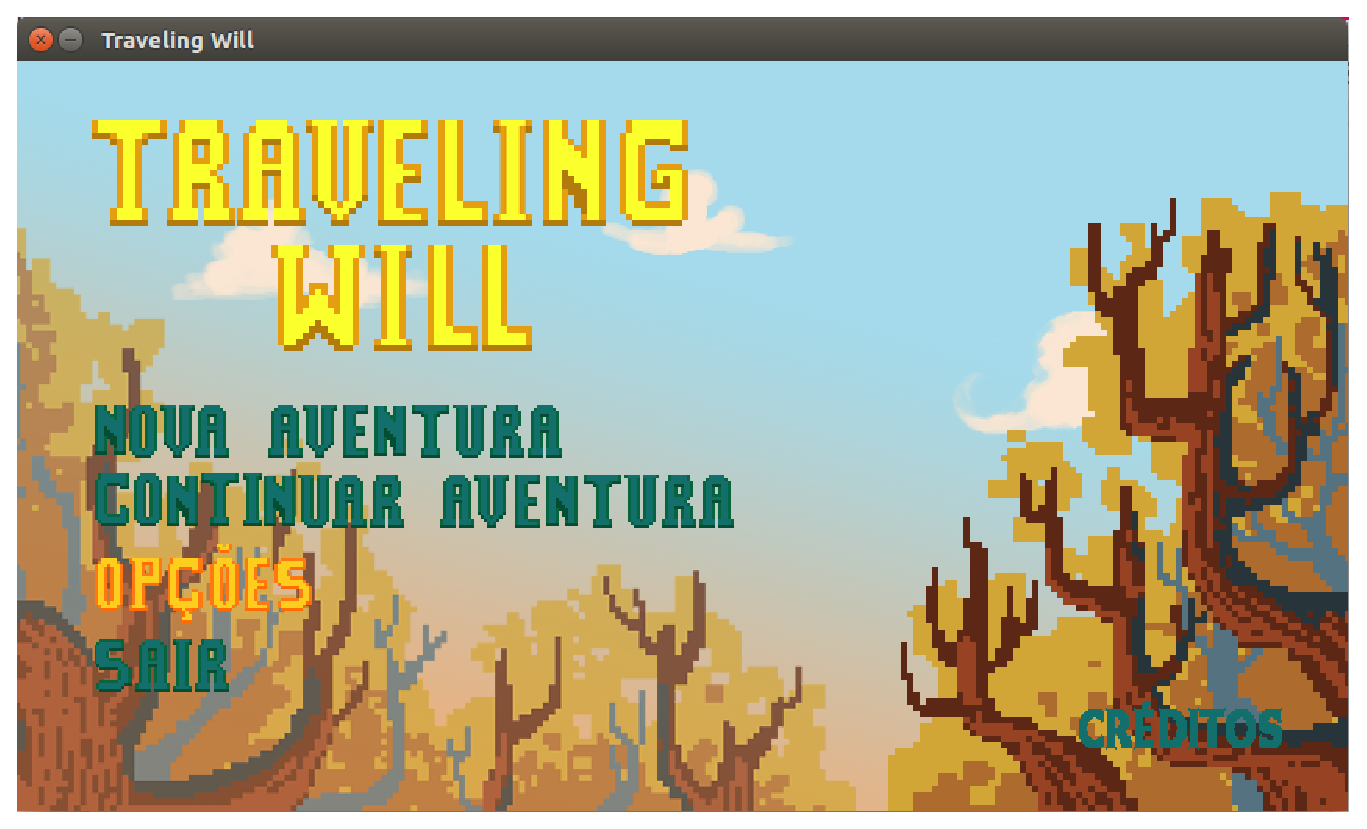
\includegraphics[width=16cm]{figuras/tw-original-1.eps} }}%
%     \qquad
%     \subfloat[Protótipo sendo executado no emulador de GBA. Fonte: \textit{Autores}.]{{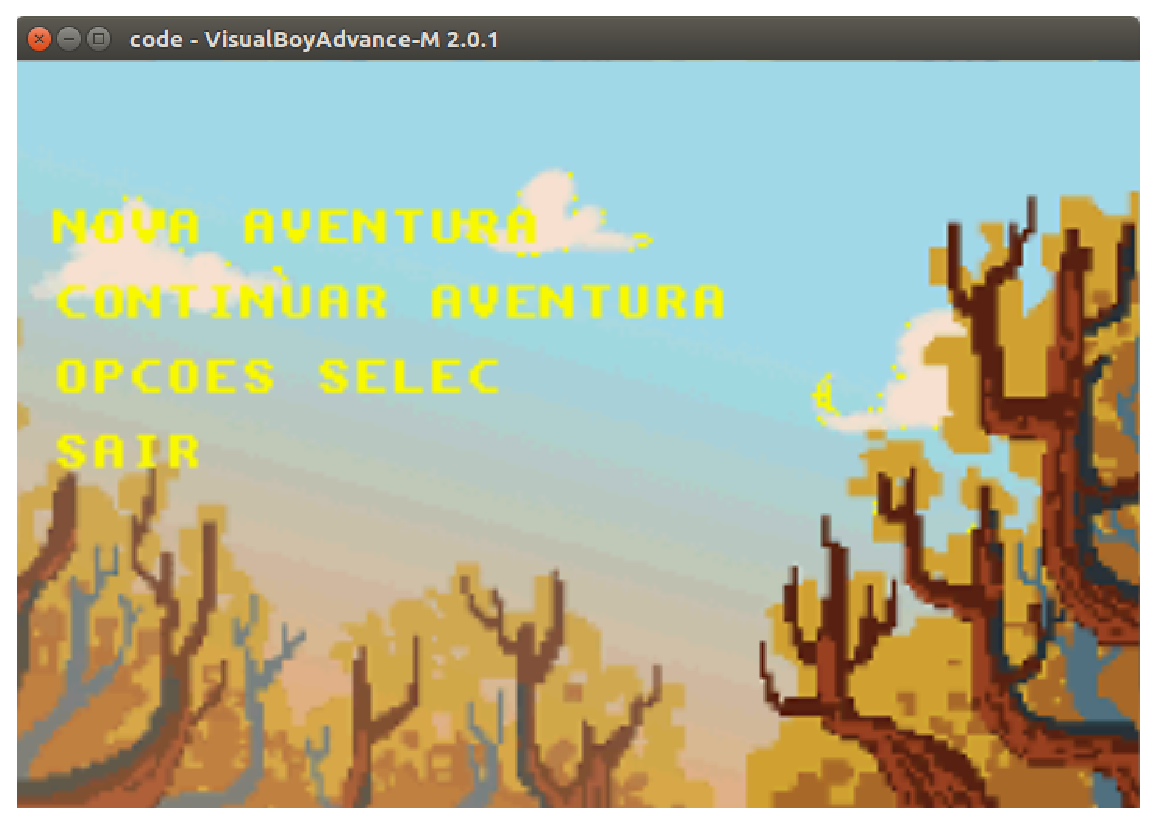
\includegraphics[width=16cm]{figuras/tw-gba-1.eps} }}%
%     \caption{Comparação entre o jogo original e o protótipo no emulador.}%
%     \label{fig:example}%
% \end{figure}

% - adaptações em relação ao jogo original
%   - não possui opção para configurar o áudio durante o jogo
%   - não possui mecanismo de salvamento de dados do jogo
%   - não possui inimigos (ainda dá)
%   - não possui seletor de fase
%     - as fases são jogadas em ordem
%     - é possível pular de fase pressionando SELECT

% - transformar as imagens do jogo (Adaptação das imagens do jogo)
%   - proporção 3:1
%   - paleta de 15 cores
%     - bit 0 transparente, mas o grit não faz isso certo
%     - especificar comandos do grit gerados para backgrounds e paletas
%   - backgrounds
%     - especificar paleta de cores na hora de gerar o grit
%     - como foi feito o scroll infinito dos backgrounds
%       - falar sobre os registradores
%   - texturas
%     - animação -> como foi feita
%     - plataformas -> uma plataforma contém várias sprites
%       - metadata.om = 2 para esconder as plataformas da tela (senão portal)
%         - colocar imagem do portal
%     - problemas com lixo na OAM, sprites espelhando

% - parse do level design (Construção de um nível do jogo)
%   - explicar como é o level design do traveling will
%   - explicar o que o parser gera e como ele é usado no jogo
%   - colocar código do parser python
%   - explicar o uso de fila para as plataformas (pouca memória)
%     - construtor por cópia
%   - velocidade das plataformas é dada pela velocidade do background mais a frente
%   - fim do level tudo para
%     - will se mexe

% - Transição entre níveis do jogo
%   - dois tipos de níveis (jogáveis e não-jogáveis)
%   - escolha do nível a ser construído
%     - switch case
%       - não era possível modularizar por causa das variáveis (inferência de nome)

% - Adaptação das músicas do jogo
%   - falar brevemente sobre os canais de áudio do gba e colocar referência
%   - falar que o módulo de áudio atual permite reproduzir notas únicas (ondas quadradas?)
%   - colocar código da reprodução da notas
%   - falar do parser do level design para extrair a música do level
%     - explicar o que ele gera
%   - colocar código do parser
%   - explicar que esse modelo não foi utilizado por era muito simples
%   - falar que o GBA consegue reproduzir apenas sons .mode
%   - falar sobre conversão de wav pra mod
%     - falar sobre a quantidade de bits do wav (colocar referência)
%     - conversão da quantidade de bits do wav
%     - conversão do wav pra mod (usando a ferramenta X)
%       - qualidade do som diminui bastante
%   - problemas em executar o nível e o áudio ao mesmo tempo
%     - sincronização da música com o level e velocidade do jogo

% - problemas gerais
%   - depuração de código
%     - rodar debuggers (gdb, etc)
%     - somente a base de print

% - o que não foi feito
%   - mixer sofisticado
%   - módulo de texto
%     - fontes bitmap mode + outras prioridades
%   - inimigos (ainda dá)